\documentclass{article}
\usepackage[utf8]{inputenc}
\usepackage{geometry}[top=2.54cm, bottom=2.54cm, left=2.54cm, right=2.54cm]
\usepackage{xcolor}
\usepackage{graphicx}
% \usepackage{subfig}
\usepackage{caption}
\usepackage{subcaption}

\usepackage{textcomp}
\usepackage{amsmath}
% \usepackage{gensymb}
% \usepackage[T1]{fontenc}

\usepackage{hyperref}

\newcommand{\degree}{\ensuremath{^\circ}}

\title{Rannsóknarskýrsla: Autonomous UAV Landing}
\author{Joshua Springer, Garret Forthofer, Kjartan Már Andersen}
\date{September 2020}

\begin{document}

\maketitle

\begin{abstract}
    We discuss the design, construction, and operation of two semi-autonomous drones during Summer 2020. The goal of the project is to develop a method for autonomously landing the drones in a target area designated by a fiducial marker and detected by a camera. We have constructed two drone platforms, and have designed and created components to adapt our ideal computational electronics to these platforms. Improvements upon similar projects include mounting the camera on a gimbal to allow a larger detection range, and using a new and computationally efficient fiducial marker system. Design choices, practical challenges, and results are presented. The drones are able to fly reliably and have nearly accomplished the goal of autonomously landing.
\end{abstract}

% \section{Overview}
% This project discusses the construction and operation of two semi-autonomous drones, with 
\section{Introduction}
Autonomous drone flight has wide-ranging applications from power line inspection to package delivery. One important aspect of autonomous drone flight that is lacking is autonomous landing, as a result of the challenges that are specific to landing in an unknown environment, such as obstacles and uneven ground. A typical method to autonomously land drones is to use computer vision and fiducial markers to identify and travel to a safe landing area.\cite{visual_servoing}\cite{high_velocity_landing}\cite{vision_based_x_platform} Fiducial markers provide a means of calculating the pose of the drone with respect to the landing pad. However these methods have not been integrated into the two main open source autonomous flight softwares: ArduPilot and PX4. These softwares offer only more primitive methods focusing on initial GPS localization and maintaining a constant rate of descent over the landing pad while performing simpler horizontal position correction based on vision. These methods are subject to GPS inaccuracies and dangers of landing even if the landing pad is not seen, meaning that the drone cannot guarantee a landing in a safe location. Other methods which have used fiducial markers typically use fixed, downward-facing cameras which can lose sight of the landing pad if the drone is not in the correct orientation, or in the final phase of landing where the drone is too close to the landing pad for the marker to be entirely in the camera's field of view.

This project provides a means of overcoming the aforementioned challenges by maintaining the drone's view of the landing pad through an automatically aimed, gimbal-mounted camera which points at the landing pad's fiducial marker throughout the entire landing, and by allowing descent only in a specific region around the landing pad. It also uses a newer fiducial marker called WhyCon \cite{whycon_paper} (shown in Figure \ref{fig:whycon}), which is more computationally efficient than the typically used April Tag \cite{apriltag_paper} (shown in Figure \ref{fig:april_tag}).

\begin{figure}
    \centering
    \begin{subfigure}[b]{0.25\textwidth}
        \centering
        
\includegraphics[width=\textwidth]{images/tag_36h11.png}
        \caption{April Tag marker.}
        \label{fig:april_tag}
    \end{subfigure}
    \begin{subfigure}[b]{0.25\textwidth}
        \centering
        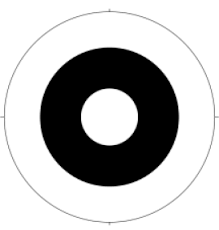
\includegraphics[width=\textwidth]{images/whycon.png}
        \caption{WhyCon marker.}
        \label{fig:whycon}
    \end{subfigure}
    \caption{Examples of fiducial markers which enable visual pose estimation.}
\end{figure}

This project involved three students: Joshua Springer and Garret Forhofer, hired as part of the RANNIS Student Innovation Fund, and Kjartan Már Andersen, hired on a summer job through Reykjavik University. The work was carried out at Reykjavik University.

\section{Methods}
In this section we describe the steps in creating a drone platform with the following properties:

\begin{itemize}
    \item The drone must be stable in manual flight and capable of autonomous flight.
    \item The drone must be capable of real-time onboard video analysis.
    \item The drone must detect a fiducial marker and track the fiducial marker by aiming a gimbal-mounted camera.
    \item The drone must approach the fiducial marker autonomously and land next to it without human intervention.
\end{itemize}

\subsection{Construction}
The Tarot 680 Pro hexacopter is the base platform selected for this project. The large (680mm radius), hexacopter design allows it to maintain its stability in relatively high winds. Its Tarot 4108 motors spin 350mm propellers which allow the drone to carry extra instruments for applications after this project. The foldable, carbon fiber frame provides structural robustness and portability. It has two batteries in order to create two isolated power systems - one for the computational and navigational electronics, and one for the propulsion system and gimbal. The power isolation prevents the motors and gimbal from causing electrical spikes which can damage or disable the computational electronics. The gimbal allows the drone to capture a stable video image over a wide angular range. 

Joshua and Garret carried out the initial construction process slowly and carefully, placing emphasis on reliability in all physical and electrical connections. This is to avoid expensive crashes by minimizing the risk of in-flight component failure. First, we mounted a motor to each of the motor arms. We soldered bullet connectors to the motor leads to attach them to the speed controllers. We mounted speed controller to the bottom of each motor mount using a 3D-printed bracket. We soldered bullet connectors to the speed controller wires, and wire extensions (also with bullet connectors) were run through the hollow arm tubes because the speed controller wires alone were too short. After all motors were verified to spin the expected direction according to the ArduPilot documentation, we placed heat shrink around all bullet connector joints for electrical insulation and physical strengthening of the connection. We assembled the drone bodies and placed the arms into their mounting points. We then fastened landing gear to the drone body. After this, we installed the computational and navigational electronics were to the mounting plate. Joshua installed the operating systems for the flight controller and companion boards, along with all necessary software (to be discussed later). ArduPilot was set up to run as a system service on the flight controller, and we carried out all necessary calibration of the accelerometers, gyroscopes, magnetometer, and RC radio according to the ArduPilot guidelines \cite{ardupilot_setup}.

% The base platform we decided to use was the Tarot 680 Pro. Construction began with individual arms, mounting the motors and their base plate to the carbon tube arms, with wires protruding from the underside. We then assembled the landing gear which was mounted with set screws into the t-joint and rubber caps place on the ends. The landing gear mount was then assembled with the tube inside, sandwiched between two mounting plates and the mount that would attach the bottom center plate of the drone. We then added the supports for the gimbal and battery mount in the form of small metal rings, which were screwed into the bottom plate, and placed rubber grommets inside them to hold the tube rails and provide them some minor dampening. plastic clips were then attached to the motor arms and mounted to the top of the bottom plate. The horizontal motor arms were not mounted with clips and would come slightly later. More clips were screwed into the top of the bottom plate such that the arms can snap into them, allowing them to fold. At this point we took all of the motor arms back off, having confirmed how they fit, and moved on to soldering them to the top board to receive power. Before we could do that, however, we needed to attach the speed controllers to the motors and arms. We first placed some heat-shrink over the wires leading out of the motors, before soldering male bullet connectors to the wire which plugs in to the speed controller. The wires from the speed controllers were not long enough to reach all the way through the carbon tube so we sourced some extra wire and used more bullet connectors and heat shrink to extend them along with a servo extension. We then trimmed the extension on the other side of the carbon tube to leave a little bit of play so that it could flex during flight and the folding of the arms before soldering them to the power board. After which, we also soldered the XT90 power connector to the board. The next process was to attach the top and bottom plates together and sandwich the final two motor arms into their metal clamps. Once that was all together, the frame was assembled and we could move on to mounting the electronics. We 3d printed another plate which sits on top of the power board in order to provide convenient mounting points for our electronics. We then mounted and connected the motors to the flight controller on their corresponding channels and then telemetry through SBUS. After testing the motors to make sure everything was configured correctly and spinning in the right direction, we then finalized our connections with the heat-shrink. We then confirmed our mounting points for the battery attached to the undercarriage of the drone with Velcro straps. The battery we are using is a 6s, 10,000mah. Now that everything has power, is configured correctly, and securely mounted, we are almost ready for the maiden flight. The only thing left to configure is telemetry and its connection to our radio transmitter. Once bound we tested the drone for the first time. *****Maybe point to the results section here***** After testing the mechanical and manual flight aspects of our drone, we could move on to configuring and mounting the gimbal and jetson-nano. The gimbal being used is a T4-3D tarot gimbal designed for the GoPro Hero 3. We designed and 3d printed a camera mount to work within these dimensions. After working with several drivers and firmware updates, everything was configured on the gimbal so we could begin manual testing. To do this we bound the gimbal to our radio transmitter. We discovered several inconsistencies with the gimbal struggling to maintain extreme angles. In response, we limited the maximum angle that it could acheive. From there the gimbal is connected to the Navio which is connected to the Jetson Nano which we now mounted to the top plate. The Navio is connected to the Jetson Nano via MAVROS over Ethernet. The Jetson Nano would then process the image from the gimbal camera and tell the Navio to provide PWM signals in order to control the gimbal to look at the April Tag or WhyCon marker. 

\subsection{Hardware Setup}
The drones have essentially the same setup, but with slightly different configurations as they use different companion boards. This section describes the systems generally, referring to the specific companion boards only when necessary.

Figure \ref{fig:hardware_setup} shows a diagram of the hardware setup for the two drones. The components and their purposes are outlined below:
\begin{itemize}
    \item \textbf{11.1 V LiPo Battery:} this battery provides power to a battery eliminator circuit (BEC) for isolation of the power system for the computational electronics (the flight controller and companion board).
    \item \textbf{BEC (Battery Eliminator Circuit):} the BEC transforms 11.1V power to 5V power for the flight controller and companion board. The flight controller and companion board each have their own 4A channel to meet their given power requirements.
    \item \textbf{Flight Controller:} this combination of a Raspberry Pi 3 B+ and Navio2 shield runs the ArduPilot software to control the drone, and communicates with the companion board to control the gimbal.
    \item \textbf{Telemetry Radio:} the telemetry radio provides two-way communication between the flight controller and a ground control station that is also fitted with its own telemetry radio. It is connected to the flight controller via USB. The software on the ground control station provides an interface for real-time status messages and sending high-level commands.
    \item \textbf{RC Receiver:} the RC receiver provides a one-way radio link between the pilot's transmitter and the flight controller, allowing the pilot to manually control the drone. It is connected to the flight controller via SBus which provides an 8-channel multiplexed PWM signal to reduce the needed wires and space. This provides an interface for control by a human pilot, which is often used in testing but will eventually be mostly unused.
    \item \textbf{22.2 V LiPo Battery:} this battery provides power to the speed controllers and gimbal.
    \item \textbf{Speed Controllers:} the speed controllers receive a PWM signal from the flight controller which indicates a throttle value. They then provide corresponding power signals to the motors.
    \item \textbf{Motors:} the motors spin propellers to provide thrust in order to control the drone's position in the air.
    \item \textbf{Gimbal:} the gimbal controls the orientation of the camera based on PWM signals from the flight controller which indicate target angles. Its onboard IMU and driver filter the motion of the camera in order to provide a smooth camera image.
    \item \textbf{Companion Board:} the companion board reads an image from the camera and calculates the position of the landing pad relative to the drone. It then communicates this information to the flight controller via an Ethernet over USB connection using ROS.
    
\end{itemize}

\begin{figure}
    \centering
    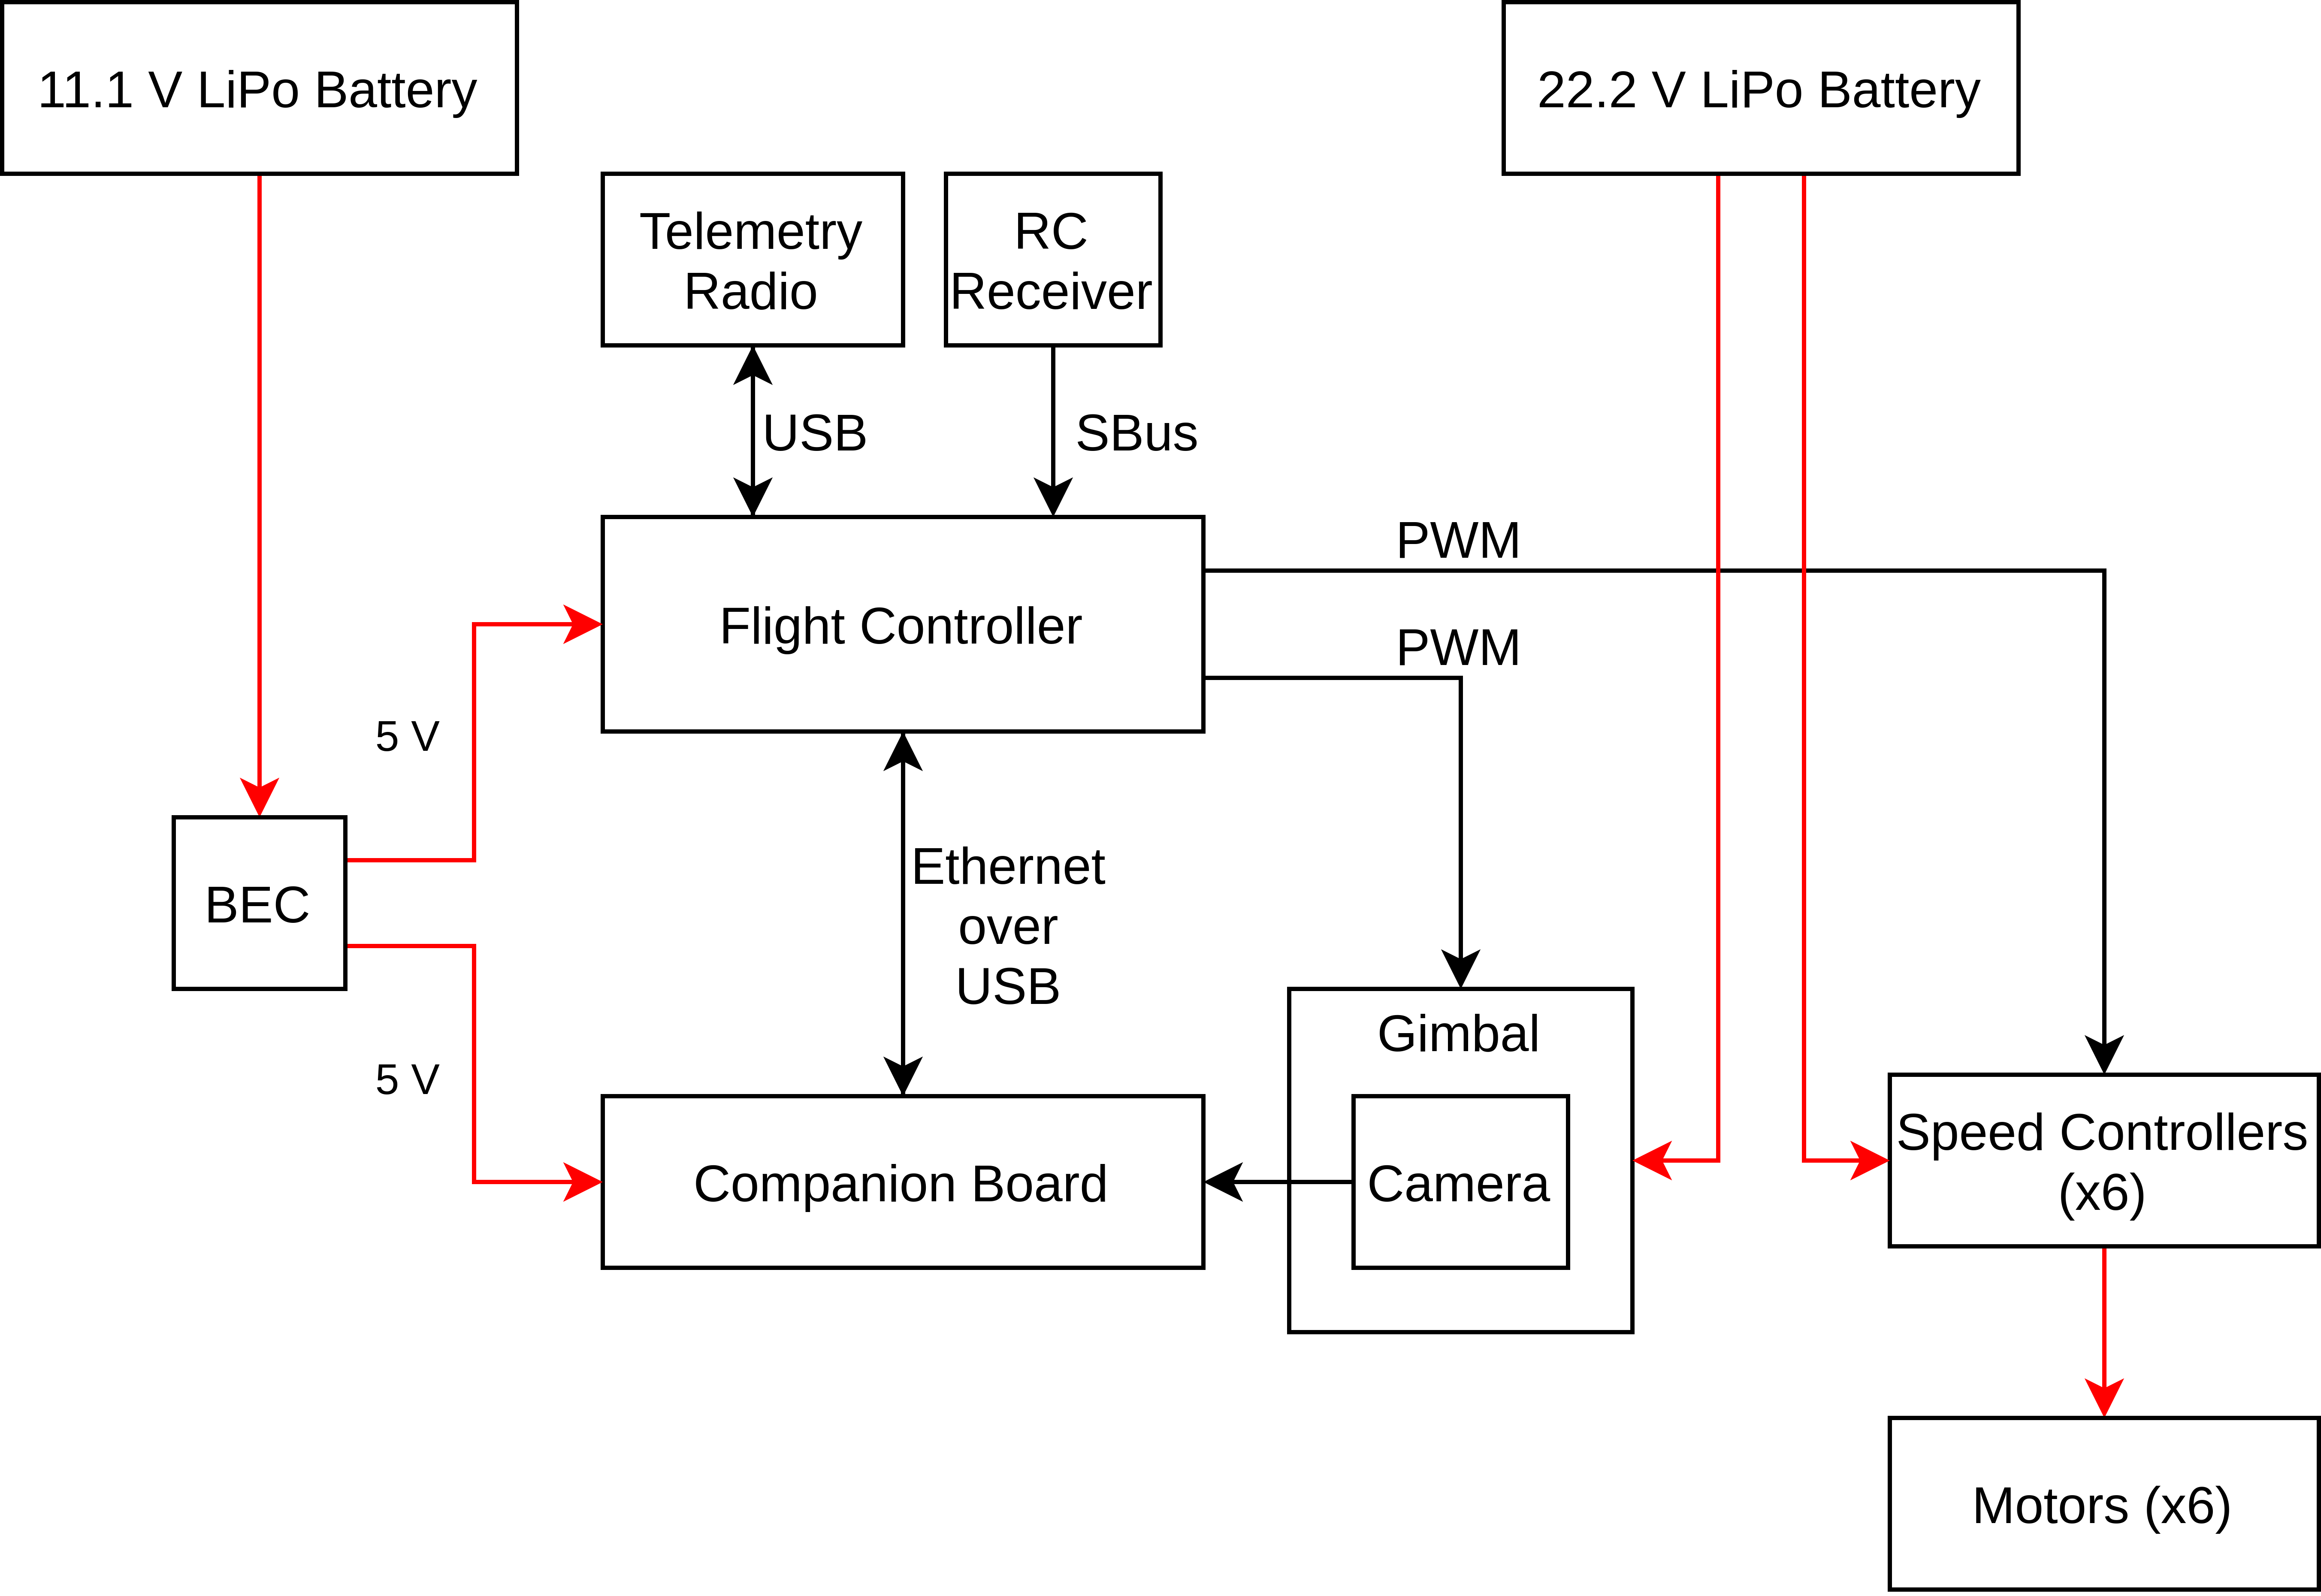
\includegraphics[width=0.8\textwidth]{images/hardware.png}
    \caption{Hardware Setup}
    \label{fig:hardware_setup}
\end{figure}

\subsection{Flight Controller Unit}

The flight controller unit (FCU) on both drones is a Raspberry Pi 3 B+ with a mounted Navio2 \cite{navio2_website} shield. The Navio2 provides inertial measurement data to the onboard autopilot software \textit{ArduPilot}, which is available open source \cite{ardupilot_website}. It runs as a system service in the Emlid distribution of the Raspbian OS, which is designed specifically for the Navio2. ArduPilot provides modes for manual, semi-autonomous, and fully autonomous flight. The ArduPilot software has \textit{not} been modified for this project. A ROS \cite{ros} module called MAVROS \cite{mavros} communicates with ArduPilot via its MAVLink \cite{mavlink_website} language in order to enable networked communication with the companion boards.

\subsection{Companion Boards}

Each drone has a second onboard processor (in addition to the flight controller), called a \textit{companion board}, the point of which is to reduce the computational load on the flight controller, which must run in real time. The companion board carries out the required video analysis, pose estimation, coordinate system transforms, and instantiates PID controllers to aim the gimbal. It then sends commands via MAVROS to the flight controller to act on this information. Connections between the companion board and the FCU are minimized in order to maintain modularity and decrease hardware and software invasiveness. Conveniently, each of the companion boards can act as a USB host, providing Ethernet over USB with static IP addresses on each end. This means that the only data connection between the companion board and the FCU is a single USB connection. Communication is established by configuring the ROS instance on the companion board to use a ROS Master instance on the FCU. This is accomplished simply by setting the \texttt{ROS\_MASTER\_URI} environment variable to the IP:port combination of the FCU, and setting the \texttt{ROS\_HOSTNAME} environment variable to the companion board's hostname. Initial setups accomplished this same configuration over a physical Ethernet connection, but the USB setup was proven more reliable given the space limitations in the drones' electronics compartments. (Physical pressure was put on the Ethernet cables when the canopy was closed, breaking the connection unpredictably.) Kjartan also tested a simulated Ethernet connection that was established from the Jetson Nano's UART port to the Raspberry Pi's USB port using two PPP services - one on the Raspberry Pi and one on the Jetson Nano. Acceptable connectivity between the boards when the services were configured to a baud rate of about 1,000,000. However, this was ultimately less reliable than using the Jetson Nano's native USB host functionality because of issues with the PPP services not syncing during boot. Using Ethernet over USB also eliminated the extra static IP configuration required with conventional Ethernet.

% An NVIDIA Jetson Nano is included on the drone in order to act as a companion board, reducing the computational requirements of the FCU. The Jetson Nano handles the image processing and coordinate system transformations that are involved in locating the landing pad via computer vision. It runs ROS modules (as system services) to carry out these tasks, and the ROS system is configured to act as a slave system to the ROS instance on the Raspberry Pi, via a single Ethernet connection. WhyCon and April Tag ROS modules analyze the image from the onboard camera to locate the fiducial markers on the landing pad. Proportional-integral-derivative (PID) controllers aim the camera directly at the markers by determining the markers' positions in the camera frame, attempting to place the markers in the center of the frame. The pan and tilt axes of the camera's gimbal are controlled by PWM signals generated by the Navio2, and the duty cycles of these signals are sent from the Jetson Nano to the Navio2, so that hardware connections from the companion board to the drone system are minimized. The channels for the gimbal tilt and pan are configured to forward the manual input signals from the drone operator to the PWM output rail, allowing the gimbal to be controlled manually during normal flight. However, when a fiducial marker is identified and the FCU is in ``Guided'' mode, this manual control is overridden using the MAVROS {\color{red} override RC in} topic. This has two principal benefits: first, the drone is able to switch between manual and automatic gimbal control, and second, the PWM connections to the gimbal are made on the FCU. This maintains modularity with respect to the companion board.

% Further, the WhyCon and April Tag ROS modules determine the positions of their respective fiducial markers in space. This allows the drone to identify and locate the landing pad, which is fitted with fiducial markers. These modules output the \textit{pose} (translation and rotation) of the fiducial markers with respect to the camera. The gimbal controller and landing controller ROS modules manipulate this pose to determine the pose of the camera with respect to the markers, and taking into considering the pan of the gimbal. Finally, three PID controllers use this information to calculate a target velocity that will direct the drone towards the landing pad. This target velocity is sent to the FCU and ArduPilot carries out all low-level commands to achieve this target velocity.



\subsection{Camera Modules and Cases}
A camera was needed for the UAV to visually identify the fiducial marker. The gimbal we used was designed for a GoPro Hero 3, but the latency of GoPro video streams meant that a GoPro would be unusable. Therefore, alternative cameras modules were used - namely, the IMX219-160 wide-angle camera and the Google Coral camera module. These allow for near realtime video streaming and analysis with the given companion boards. Kjartan and Joshua iteratively designed and tested multiple camera cases (shown in Figure \ref{fig:camera_case_iterations}) to properly mount the camera modules in the gimbal's GoPro holder. We then 3D printed them and installed them on the drones. According to the gimbal's design, the lens of the GoPro is supposed to be slightly off-center in both the horizontal and vertical directions. In early versions of the camera cases, the camera modules were positioned in the same place. This meant that the modules would have to be rotated 90 degrees in order to allow their data cables to extend out of a small slit the case without obstruction. The video feed was then rotated back before video analysis. However, in later revisions of the camera cases, we have positioned the lenses closer to the center of rotation in the pan and tilt axes. This allows room for the camera's ribbon cable to extend out of the bottom of the camera case without obstruction, creates a neater and more reliable system, and eliminates the need for rotating the video feed in software. The final camera modules are shown in Figures \ref{fig:nano_case} and \ref{fig:coral_case}. They were designed in OpenSCAD and all .stl and .scad files are available freely on Thingiverse \cite{camera_thingiverse}.

\begin{figure}
    \centering
    \includegraphics[width=0.7\textwidth, angle=180]{images/camera_module_iterations.JPG}
    \caption{Iterations of the camera case design The camera module was gradually moved to the side and oriented upwards in order to allow the best fit in the gimbal.}
    \label{fig:camera_case_iterations}
\end{figure}

\begin{figure}
    \begin{subfigure}[b]{0.48\textwidth}
        \centering
        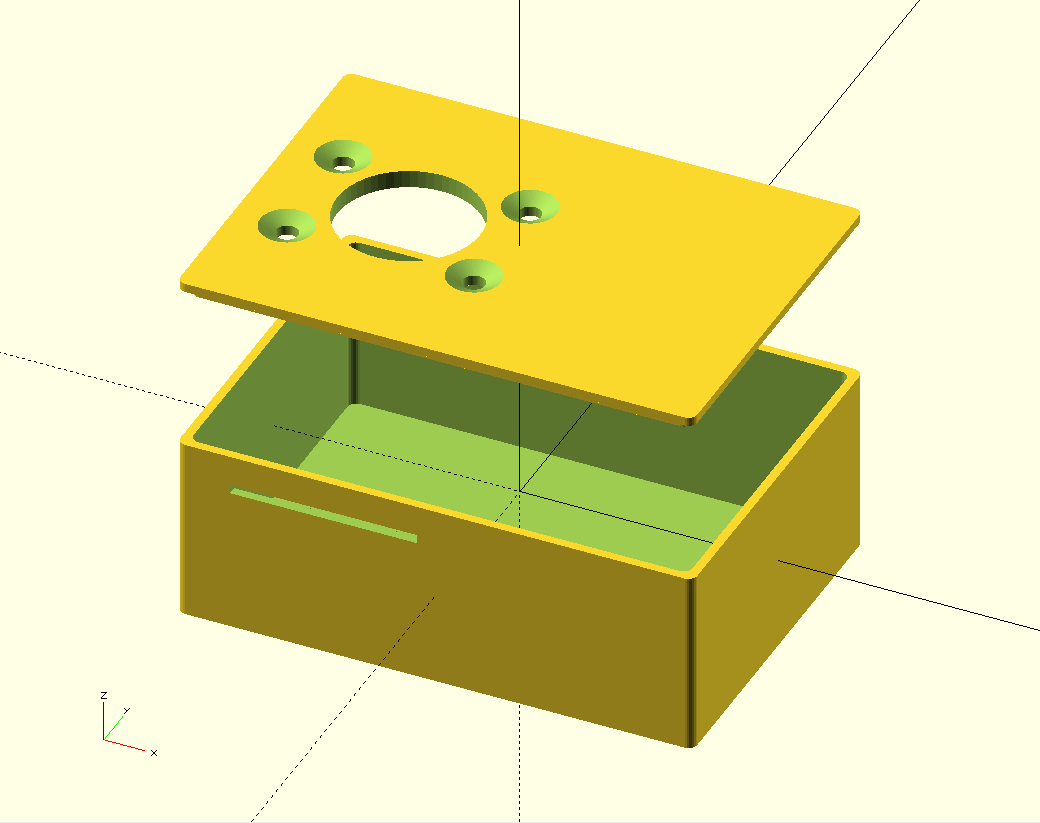
\includegraphics[width=\textwidth]{images/nano_case.png}
        \caption{The case for the IMX219-160 camera module.}
        \label{fig:nano_case}
    \end{subfigure}
    \begin{subfigure}[b]{0.48\textwidth}
        \centering
        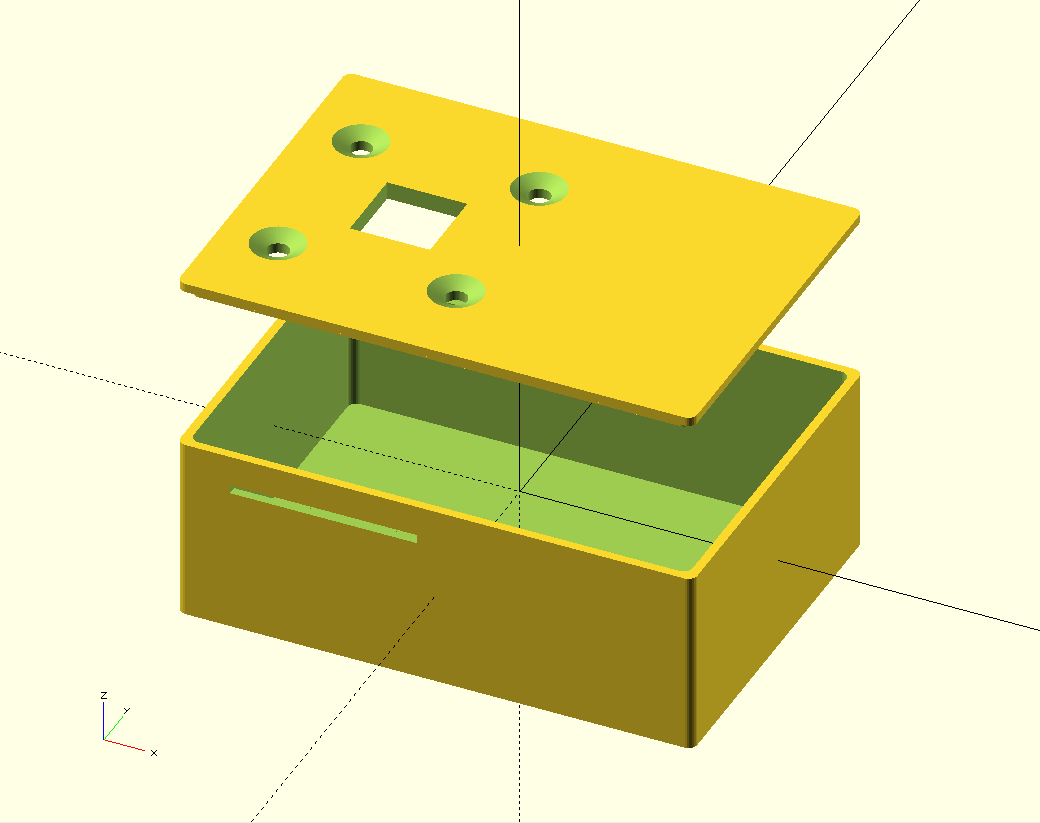
\includegraphics[width=\textwidth]{images/coral_case.png}
        \caption{The case for the Google Coral camera module.}
        \label{fig:coral_case}
    \end{subfigure}
    \caption{Cases to allow the alternative camera modules to fit into the gimbal's GoPro mount. The camera modules mount to the front with screws, and the front simply presses into the back. A slit allows the camera's ribbon cable to exit the bottom of the case.}
\end{figure}



% In order to use the module, we designed an empty camera case based on the dimensions of the Hero 3 and put the module inside the case. Four screw holes were added to the top cover of the case for the module to be screwed into, and a hole in the middle of the screw holes for the lens to go through. Enclosures were added to the case to snap the top cover and the case together. A component of the gimbal that would fasten a GoPro Hero 3 to the gimbal was removed so we could use our case instead, and because the component would be in the way of the camera's vision. We used Fusion 360 to design the case, and used Ultimaker Cura to slice the model for 3D printing. After we had 3D printed the case and tested the camera, we came to the conclusion that a much wider lens would be more optimal. We designed a new top cover but did not redesign the rest of the case since the only thing we were changing was a new camera module. 

\subsection{Component Mounting Plate}
In initial tests, basic components were mounted to the drone using simple mounting tape. In later tests, a more robust solution was required. Because of the specific component set, Joshua created a lightweight mounting plate to accommodate both the components and an overhead canopy. A canopy designed for the Tarot 680 was conveniently available directly on Thingiverse \cite{canopy_thingiverse}, and it provides physical protection of the onboard electronics from moisture, dust, and other debris. A mounting plate for the components (shown in Figure \ref{fig:component_mounting_plate}) was designed to fit the top plate of the drone. It mounts using screws in the unused holes in the top of the drone's plate. Larger screw holes allow the plate to sit flush against the drone's top plate even with the existing screws which stick up slightly. These screws also help to keep the mounting plate in place laterally. Larger central holes allow wires to pass through the plate from the center to the electronics. Standoffs provide a well-organized and stable mounting point for the flight controller and companion boards. The vertical plates on the side provide a mounting place for the RC receiver and BEC. The hinge in the back connects to the corresponding hinge on the canopy, and the slit in the front allows a Velcro strap to hold the canopy closed. The hole in the canopy allows the GPS antenna to be mounted externally. An additional hole was made to accommodate the antenna for the telemetry radio. A specific mounting plate was created for each drone because the mounting holes for the companion boards are different, but the mounting plates are otherwise the same. The mounting plates and canopies were printed and installed on the drones iteratively, with slight changes each time. This was designed in OpenSCAD and all .stl and .scad files are available on Thingiverse \cite{mounting_plate_thingiverse}.

\begin{figure}
    \centering
    \includegraphics[width=0.7\textwidth]{images/mounting_plate_iterations.JPG}
    \caption{Iterations of the mounting plate design. The mounting plate was changed over time to be more lightweight and allow flexible placement of data and power cables.}
    \label{fig:mounting_plate_iterations}
\end{figure}

\begin{figure}
    \begin{subfigure}[b]{0.48\textwidth}
        \centering
        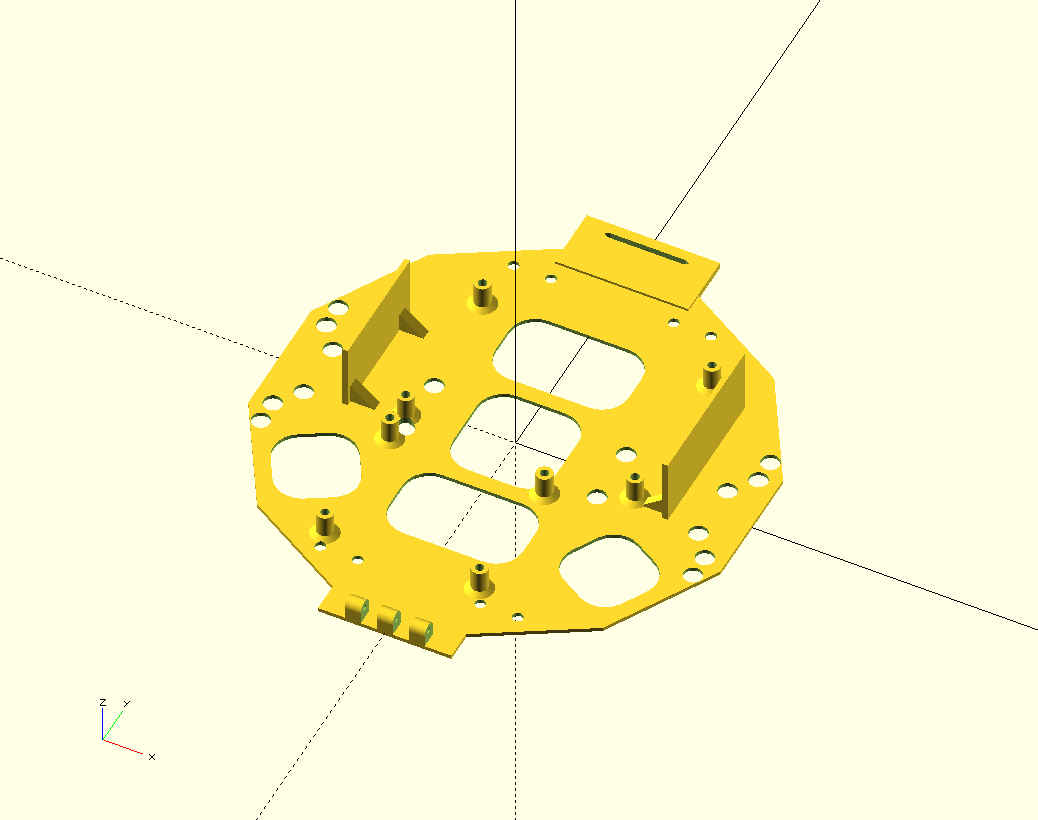
\includegraphics[width=\textwidth]{images/component_mounting_plate.png}
        \caption{Component mounting plate.}
        \label{fig:component_mounting_plate}
    \end{subfigure}
    \begin{subfigure}[b]{0.48\textwidth}
        \centering
        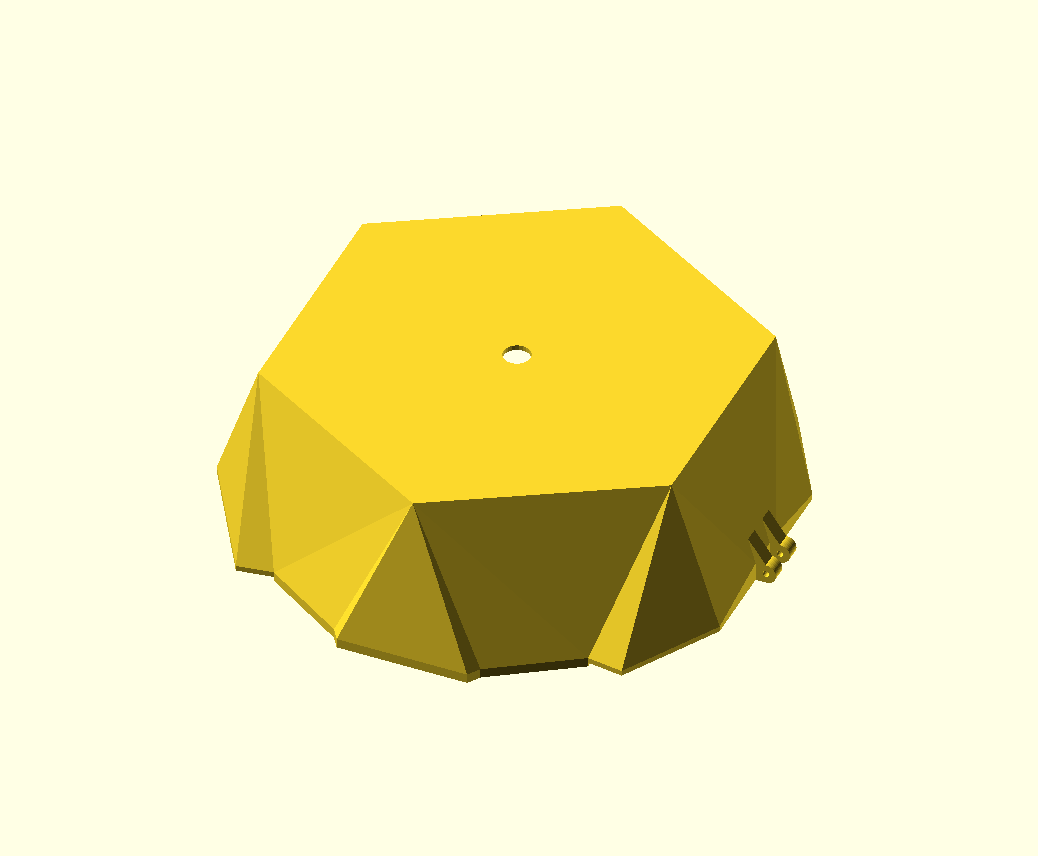
\includegraphics[width=\textwidth]{images/canopy.png}
        \caption{The canopy top for the electronics.}
        \label{fig:canopy}
    \end{subfigure}
    \caption{The final mounting plate and canopy cover.}
    \label{fig:mounting}
\end{figure}

\subsection{Software Adaptation}
This project represents the physical adaptation of an autonomous landing solution developed in simulation in \cite{AL_thesis}. The first phase of software development in this project was the adaptation of this software from the simulation environment to the physical drone system.

\begin{figure}
    \centering
    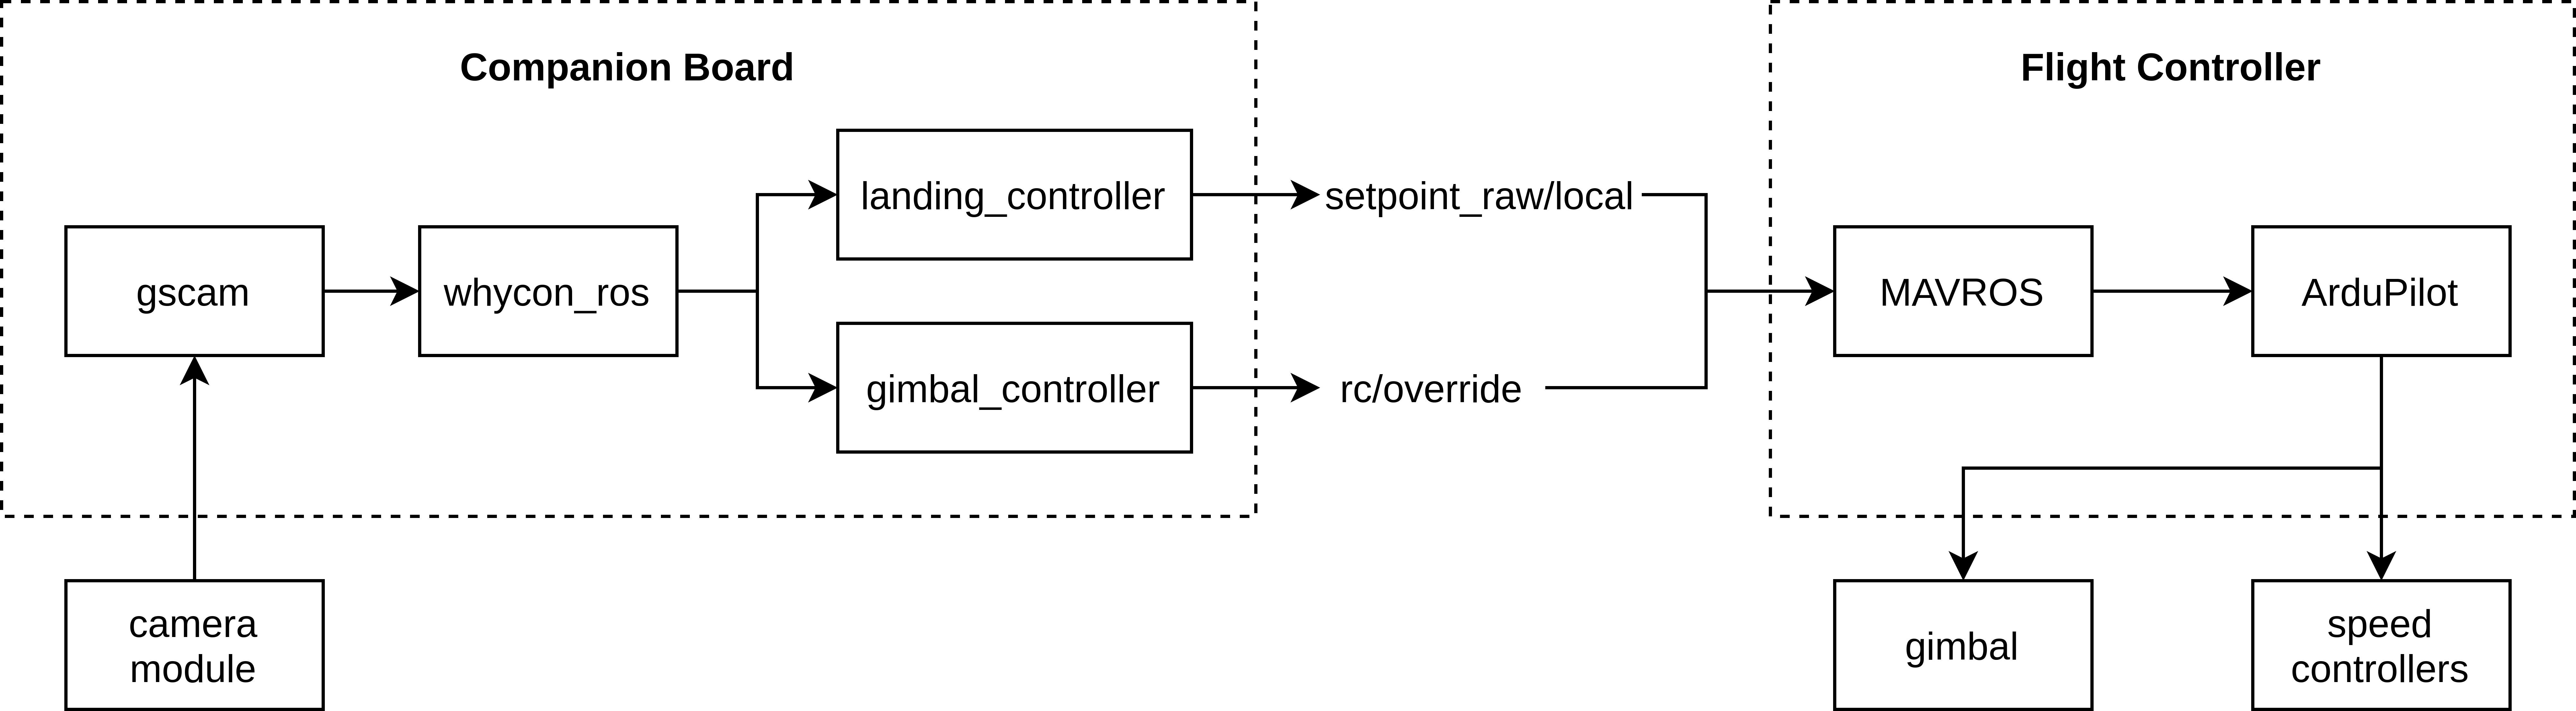
\includegraphics[width=\textwidth]{images/data_flow.png}
    \caption{Data flow.}
    \label{fig:data_flow}
\end{figure}

\subsubsection{Video Input Processing}

The Gazebo simulator in which this software was originally tested and developed provides simulated camera modules which natively provide images as a ROS topic. Joshua and Kjartan replicated this functionality with physical camera modules. This was done with a ROS package called \texttt{gscam} \cite{gscam_github}, which is designed for this functionality and acts as an interface between GStreamer (a tool for manipulating video and music files) \cite{gstreamer_website} and ROS. On the Google Coral, this was accomplished simply by using the \texttt{gscam} module alone, and on the NVIDIA Jetson Nano, this was accomplished using \texttt{gscam} and an extension to it which is called \texttt{jetson\_csi\_cam} \cite{jetson_csi_cam_github}. The \texttt{gscam} works with GStreamer pipelines, which allow simple video manipulation such as rotation and resizing, and ultimately stream the image to ROS as an image topic.

Initial tests shows an extremely high computation load and low framerate when identifying a WhyCon marker from the camera stream at full resolution. In order to reduce the computational requirements of the video analysis, the video stream is first resized by GStreamer to a manageable 640x480 resolution, from the native resolutions of 3280x2464 and 2582x1933 for the Jetson and Coral camera modules respectively. The 640x480 resolution allowed the video to be analyzed at about 30 frames per second, however this parameter is not necessarily optimal and could be changed in the future. It provided a significant performance boost over the native resolutions which allowed only a very slow analysis framerate. In the earlier revisions of the camera module cases, the video was also rotated to the correct orientation using the GStreamer pipeline before analysis.

The camera's intrinsic matrix and distortion coefficients were found through the typical ``chessboard'' calibration method using the ROS \texttt{camera\_calibration} module \cite{ros_camera_calibration} which is outlined in the original thesis \cite{AL_thesis}. The Google Coral's camera module has significantly less distortion than the Jetson Nano's wide-angle camera module because of its smaller field of view (84\degree vertically and 87.6\degree horizontally). The Jetson Nano's camera module has a field of view of 160\degree diagonally. Its large field of view makes it easier to detect fiducial markers at close range.

\subsubsection{WhyCon Adaptation}
\label{section:whycon_adaptation}

The original landing software, tested in simulation, used both April Tag and WhyCon fiducial markers, but only WhyCon is used on the physical systems in order to reduce computational load on the companion board. For context, the April Tag module was only added for reliable estimation of the yaw (rotation in the z-axis) of the landing platform, as there is some issue in determining the yaw orientation of WhyCode markers (outlined in the original thesis \cite{AL_thesis}). 

The \texttt{whycon\_ros} module from LCAS \cite{whycon_github} was only slightly modified for use in this project, and the modifications are listed below:

First, the pixel positions $u,v$ for the center of the marker were populated as part of the WhyCon/Marker message. The $u \in [0, 640]$ corresponds to the marker's $x$ position in the resized camera frame, and $v \in [0, 480]$ corresponds to the marker's $y$ position in the resized camera frame. These pixel positions allow the gimbal controller to aim the camera directly at the marker with fewer calculations than in the original software, since the pixel offset of the marker from the center of the camera's field of view corresponds roughly to physical angle offset between the marker's position and the camera's rotation in space.

Second, an additional message attribute called \texttt{theta}, in the message definition, (hereafter referred to as $\theta$) describes the $z$-axis rotation of the marker in space according to the pixel placement of its white and black regions. The centers of the white and black regions are not published as topics by the module, but they are used in other calculations and are therefore easily available in the code. If the black segment has center $u_b,v_b$ and the white segment has center $u_w,v_w$, then $\theta$ is calculated as follows:

$$\theta_i = arctan\left(\frac{v_w - v_b}{u_w - u_b}\right)$$
$$\theta = \begin{cases}
    \theta_i + \frac{\pi}{2} &\mbox{if } \theta_i \leq \frac{\pi}{2} \\
    \theta_i - \frac{3\pi}{2} &\mbox{if } \theta_i > \frac{\pi}{2}
\end{cases}$$

Then $\theta$ is the angle from the center of the marker to the center of its white region. This helps to reduce some confusion that results from rotationally symmetric markers, such as 2-bit WhyCode markers with IDs 1 and 2, shown in Figures \ref{fig:whycode_1} and \ref{fig:whycode_2}, in that orients the marker with respect to the extended white region. In Figure \ref{fig:whycode_1}, $\theta = -\frac{\pi}{2}$, and in Figure \ref{fig:whycode_2}, $\theta = \frac{\pi}{2}$. This provides a reliable yaw orientation value for the marker, but ultimately did not solve the issue discussed in Section 3.3.1 of the original thesis \cite{AL_thesis}. 

\begin{figure}
    \centering
    \begin{subfigure}[b]{0.3\textwidth}
        \centering
        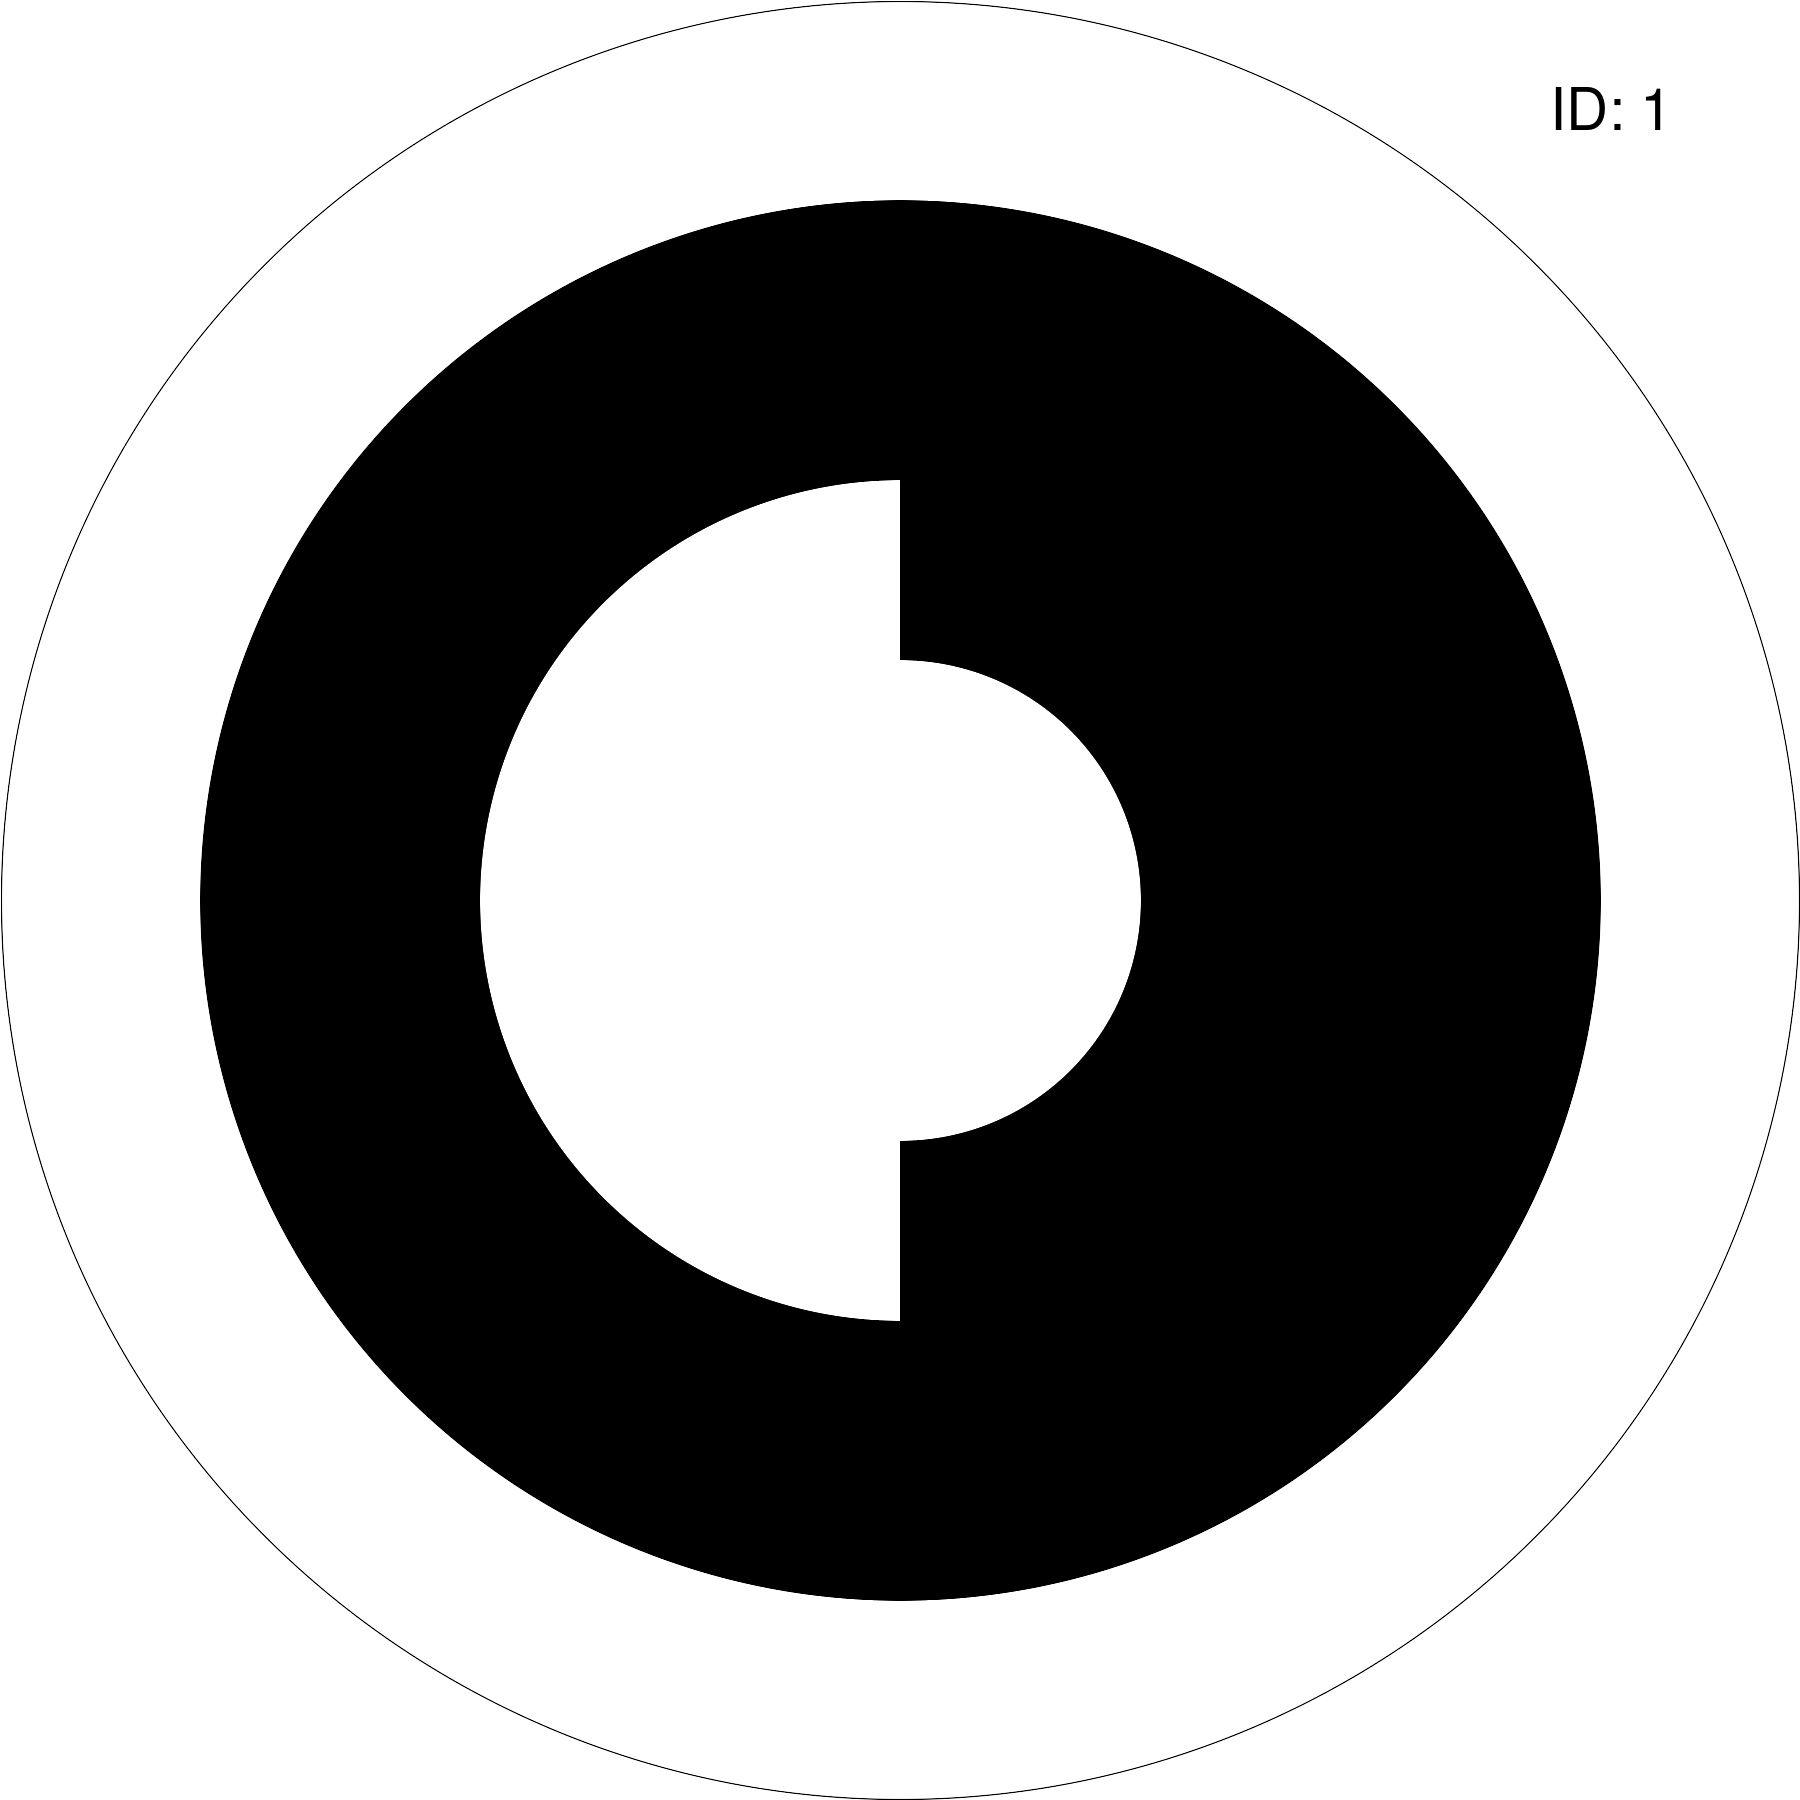
\includegraphics[width=\textwidth]{images/00000001.png}
        \caption{ID: 1}
        \label{fig:whycode_1}
    \end{subfigure}
    \begin{subfigure}[b]{0.3\textwidth}
        \centering
        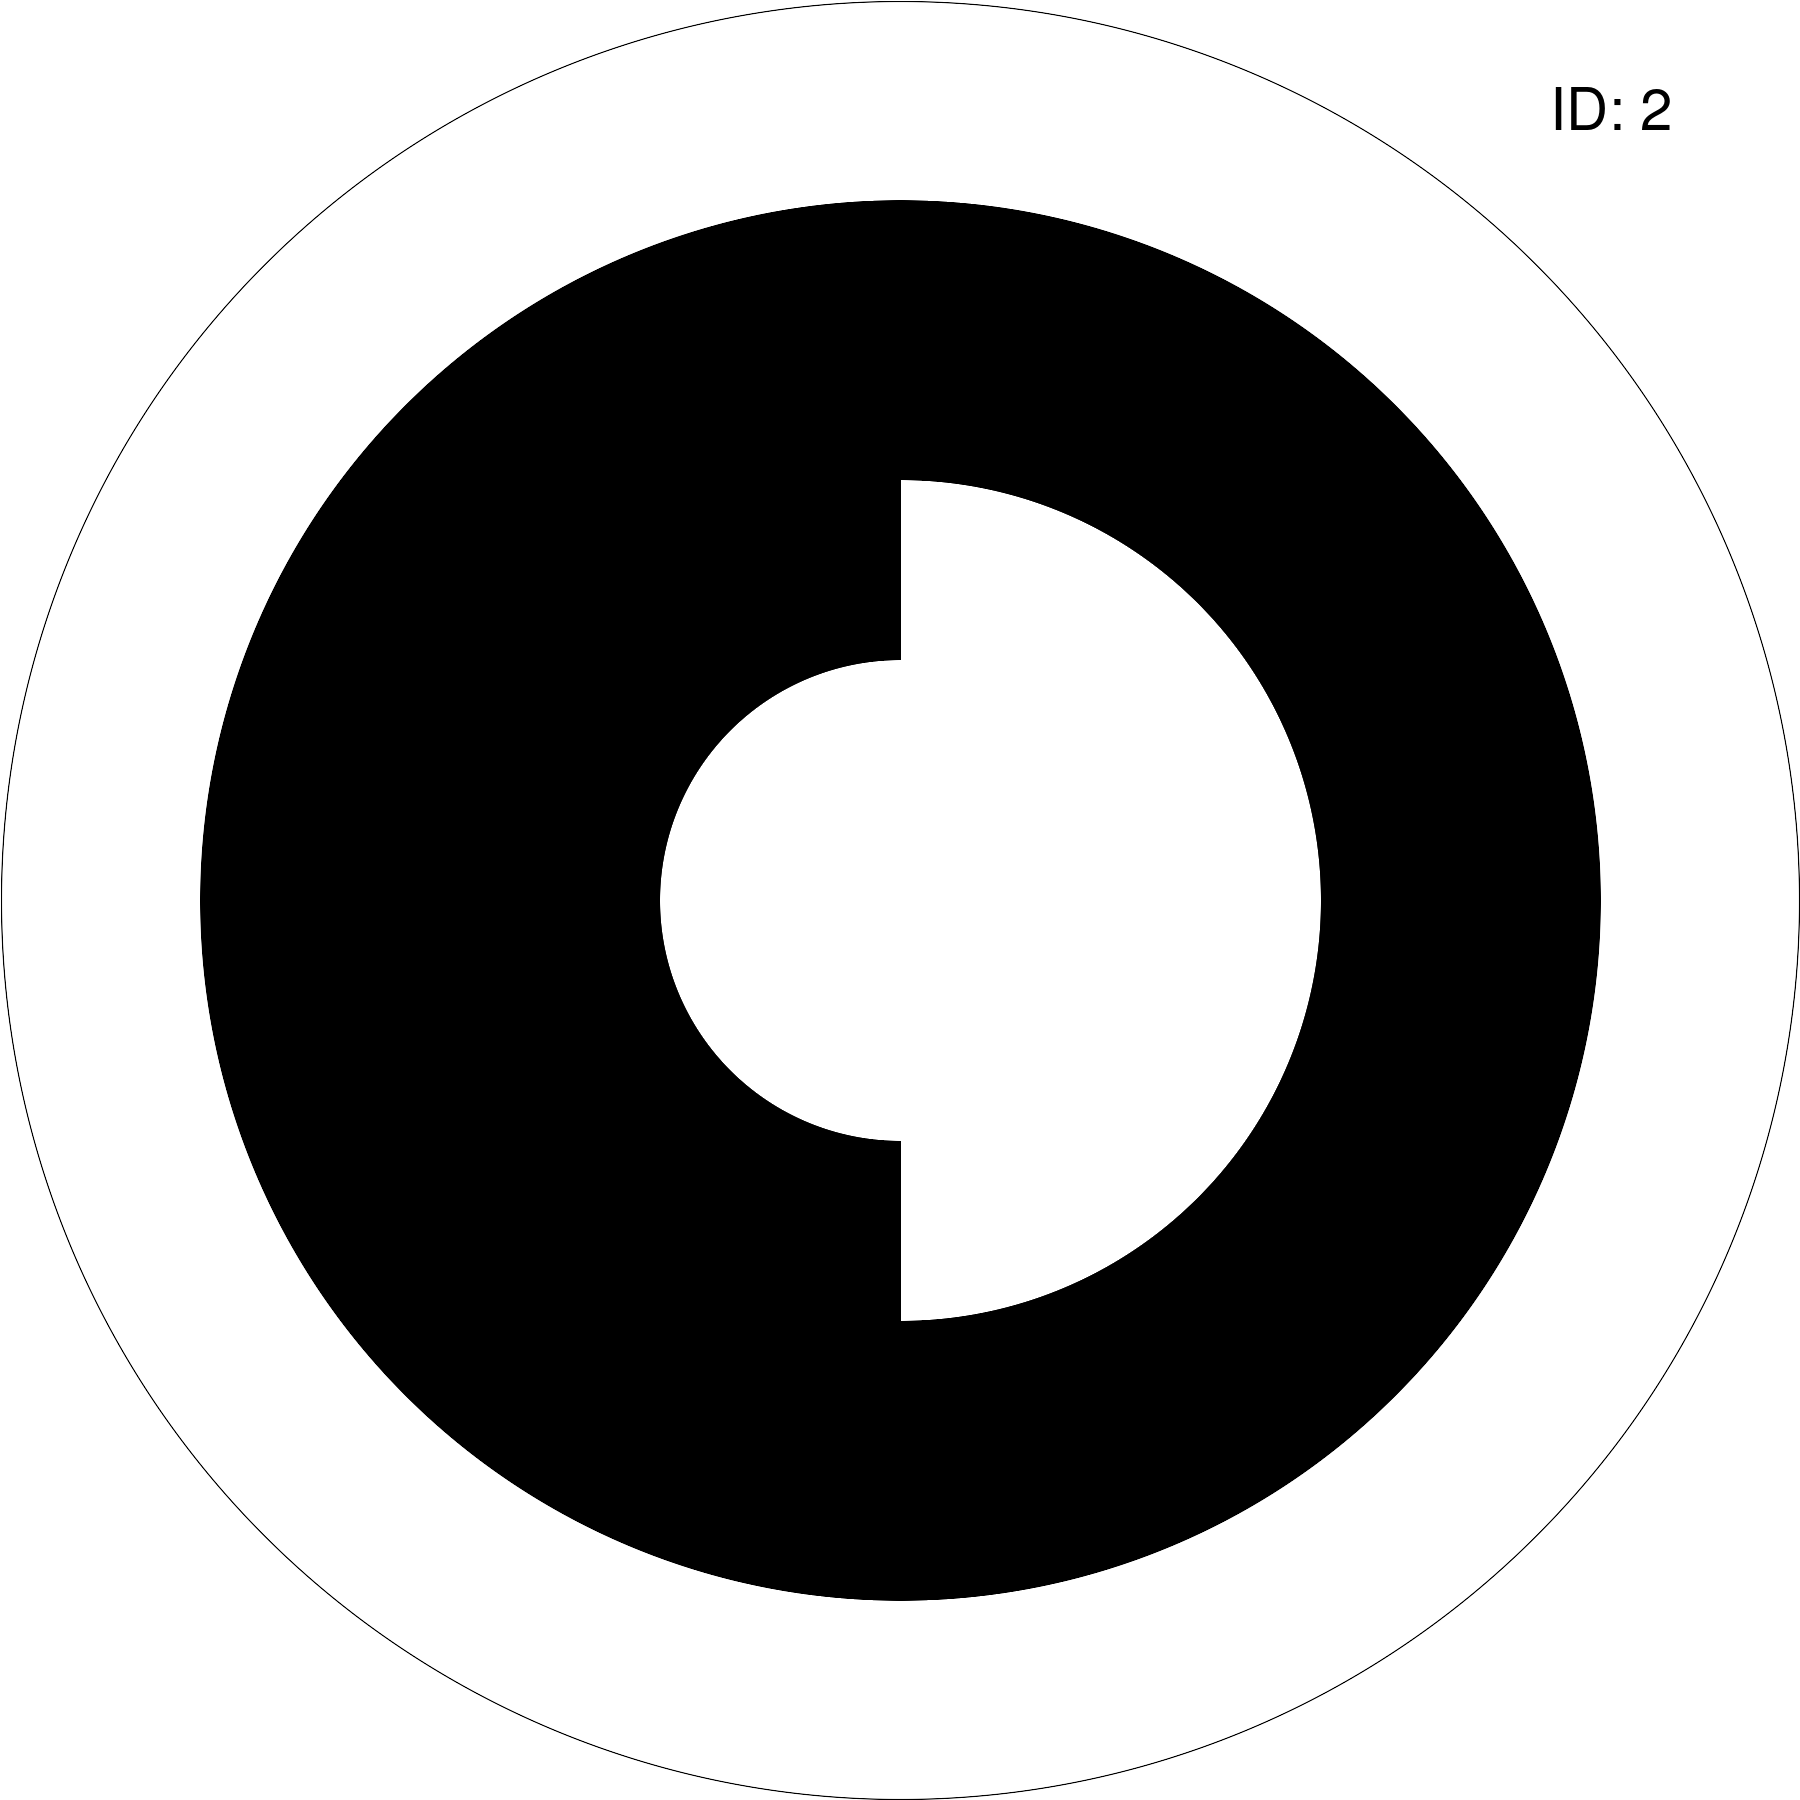
\includegraphics[width=\textwidth]{images/00000002.png}
        \caption{ID: 2}
        \label{fig:whycode_2}
    \end{subfigure}
    \caption{Rotationally symmetric WhyCode markers.}
    \label{fig:rotationally_symmetric WhyCode markers.}
\end{figure}

\subsubsection{Gimbal Controller Adaptation}
\label{section:gimbal_controller_adapation}
The gimbal controller ROS module \cite{gimbal_controller_github} has been simplified from the original simulation-tested code, in order to account for a simplified fiducial marker system. The original fiducial marker system included both a WhyCon and April Tag marker. However, in lab testing, running both fiducial systems was excessively processor intensive, typically requiring more than 50\% of CPU time, and so the April Tag marker was abandoned. The WhyCon marker alone used required less than 10\% of CPU time, although further analysis was outside the scope of this project. Overall, the purpose of the gimbal controller is to center the WhyCon marker in the camera frame by changing the pan and tilt angles of the gimbal using the pixel coordinates $u,v$ of the detected WhyCon marker.

PID controllers provide a simple means of smoothly controlling actuators.\cite{pid_control} Two PID controllers generate control effort signals which determine the rotation of the gimbal in its two axes. They take as state inputs the normalized values of $u,v$ which are $u_n, v_n \in [-1,1]$ and both have constant set points (target state values) of 0. They generate control efforts in the interval $[-1, 1]$, which are then converted to pulse width modulation (PWM) signals. These are standard signals for servo control. The gimbal controller module sends these PWM signals to ArduPilot via the MAVROS OverrideRCIn topic, and the flight controller generates the actual PWM signals on its servo output rail, controlling the gimbal.

One of the challenges in using this setup is that the true angle of the gimbal is not known, as the gimbal does not expose this information. The angles are estimated based on the known minimum and maximum angles of the gimbal which can be set in firmware. The angles can be estimated through linear interpolation from the control effort PWM signal to the angular range of the gimbal in some axis. Using, for example, the pan axis: if the control effort PWM signal is $\mathrm{PWM}_\mathrm{pan} \in [1000, 2000]$, and the pan angle $\theta_\mathrm{pan} \in [-30, 30]$, then $\theta_{pan}$ is calculated as in Equation \eqref{equation:theta_pan}:

\begin{equation}
    \theta_\mathrm{pan} = -30 + \frac{(\mathrm{PWM}_\mathrm{tilt} - 1000)(2000 - 1000)}{30 - (-30)}
    \label{equation:theta_pan}
\end{equation}

This is only an estimate of the pan angle because the gimbal controller itself implements PID controllers in all of its axes, meaning that the angle of the gimbal does not directly correspond to the control signal when the entire gimbal is turning relative to its tilt axis. This happens when the drone has some non-zero yaw velocity. We reduced this effect by commanding the drone to maintain its yaw position throughout the course of landing.

\subsubsection{Landing Controller Adaptation} 

The purpose of the landing controller ROS module \cite{landing_controller_github} is to use the information from the gimbal controller to direct the drone towards the landing pad. Joshua adapted the landing controller from the original version, which uses velocity targets, to a simpler version using positional targets. The landing controller uses the estimated relative pose of the landing pad's WhyCon marker as a positional target. In order to calculate the positional target, the landing controller transforms the WhyCon marker's relative pose using transforms generated by the gimbal controller, which take into account the 2-dimensional rotation (in the pitch and roll axes) as well as the yaw of the gimbal.  When the landing controller detects that the drone is in "GUIDED" mode and the motors are armed, then the landing controller is enabled and publishes positional targets to the \texttt{setpoint\_raw/local} topic of MAVROS, which then relays the positional target to ArduPilot. The positional target is the 3-dimensional displacement of the drone from the landing pad. It also has a positional offset in the ``north'' (front) axis, meaning that the drone should land not directly on top of the marker, but rather offset slightly in one direction. This allows the drone to track the marker throughout its entire descent because the camera never gets prohibitively close to the marker, so the marker always fits in the camera's field of view. Similar projects have attempted to land directly on top of the marker, which causes the marker to exceed the camera's field of view and close distances and become undetectable. Since the WhyCon marker has no inherent yaw orientation, no target yaw of the drone is considered. This means that the drone can land around the landing pad with a radius determined by its target positional offset in the north axis. Landing on a radius around the landing pad, instead of on a specific point, is not ideal. In future work, a WhyCode marker will be used. This is a necessary first step due to limitations on detecting the yaw of WhyCode markers, which is discussed in Section 3.3.1 of the original thesis \cite{AL_thesis}.

\subsection{Landing Pad}
After the software was adapted to the physical drone systems, a large WhyCon marker was printed as a landing pad, as shown in Figure \ref{fig:landing_pad}. It was then attached to a piece of plexiglass for rigidity. The paper unfortunately does get dirty and absorbs moisture and must therefore be replaced from time to time. This method reduces glossiness and glare on the landing platform, and provides exactitude in the shape of the marker, as opposed to painting the marker by hand.

\begin{figure}
    \centering
    \includegraphics[width=0.5\textwidth]{images/landing_pad.JPG}
    \caption{The landing pad.}
    \label{fig:landing_pad}
\end{figure}

\section{Results}

\subsection{Assembled Drones}
Figures \ref{fig:jetson_drone} and \ref{fig:coral_drone} show the fully assembled drones with the Jetson Nano (referred to as the Jetson drone) and Google Coral (referred to as the Coral drone) respectively. The two different companion boards were deliberately chosen in order to provide some comparison between the available systems. Figures \ref{fig:jetson_electronics} and \ref{fig:coral_electronics} show the electronics compartments of the drones. All electronics components in each drone are the same except for the companion boards, camera modules, and the relevant cables. These pictures show the placement of all of the components and their connections, as well as the size difference between the Jetson Nano and the Google Coral. Although the Jetson Nano was ultimately squeezed into the electronics compartment, its large size meant that it required most of the space on the mounting plate. Its fan also extended vertically to nearly the top of the canopy. The consequences of this are discussed in Section \ref{section:jetson_nano_power_consumption_and_form_factor}. By contrast, the Google Coral's smaller form factor (essentially the same as the Raspberry Pi) allows it to fit nicely, leaving even more room for additional components and airflow. The BEC provides a static DC source which generates a magnetic field, and as such it was placed as far away as possible from the compass and GPS receiver (the black case on top of the canopy. The antenna for the telemetry radio extends vertically out of the canopy, while the antennas for the RC receiver extend partially around the circumference of the canopy. The space limitations mean that there is a lot of potential for electrical and radio interference among the components. However, the different radio bands used by the components, as well as the little available physical separation that was achieved through the placement of the components, provide adequate performance during tests.

\begin{figure}
    \begin{subfigure}[b]{0.48\textwidth}
        \centering
        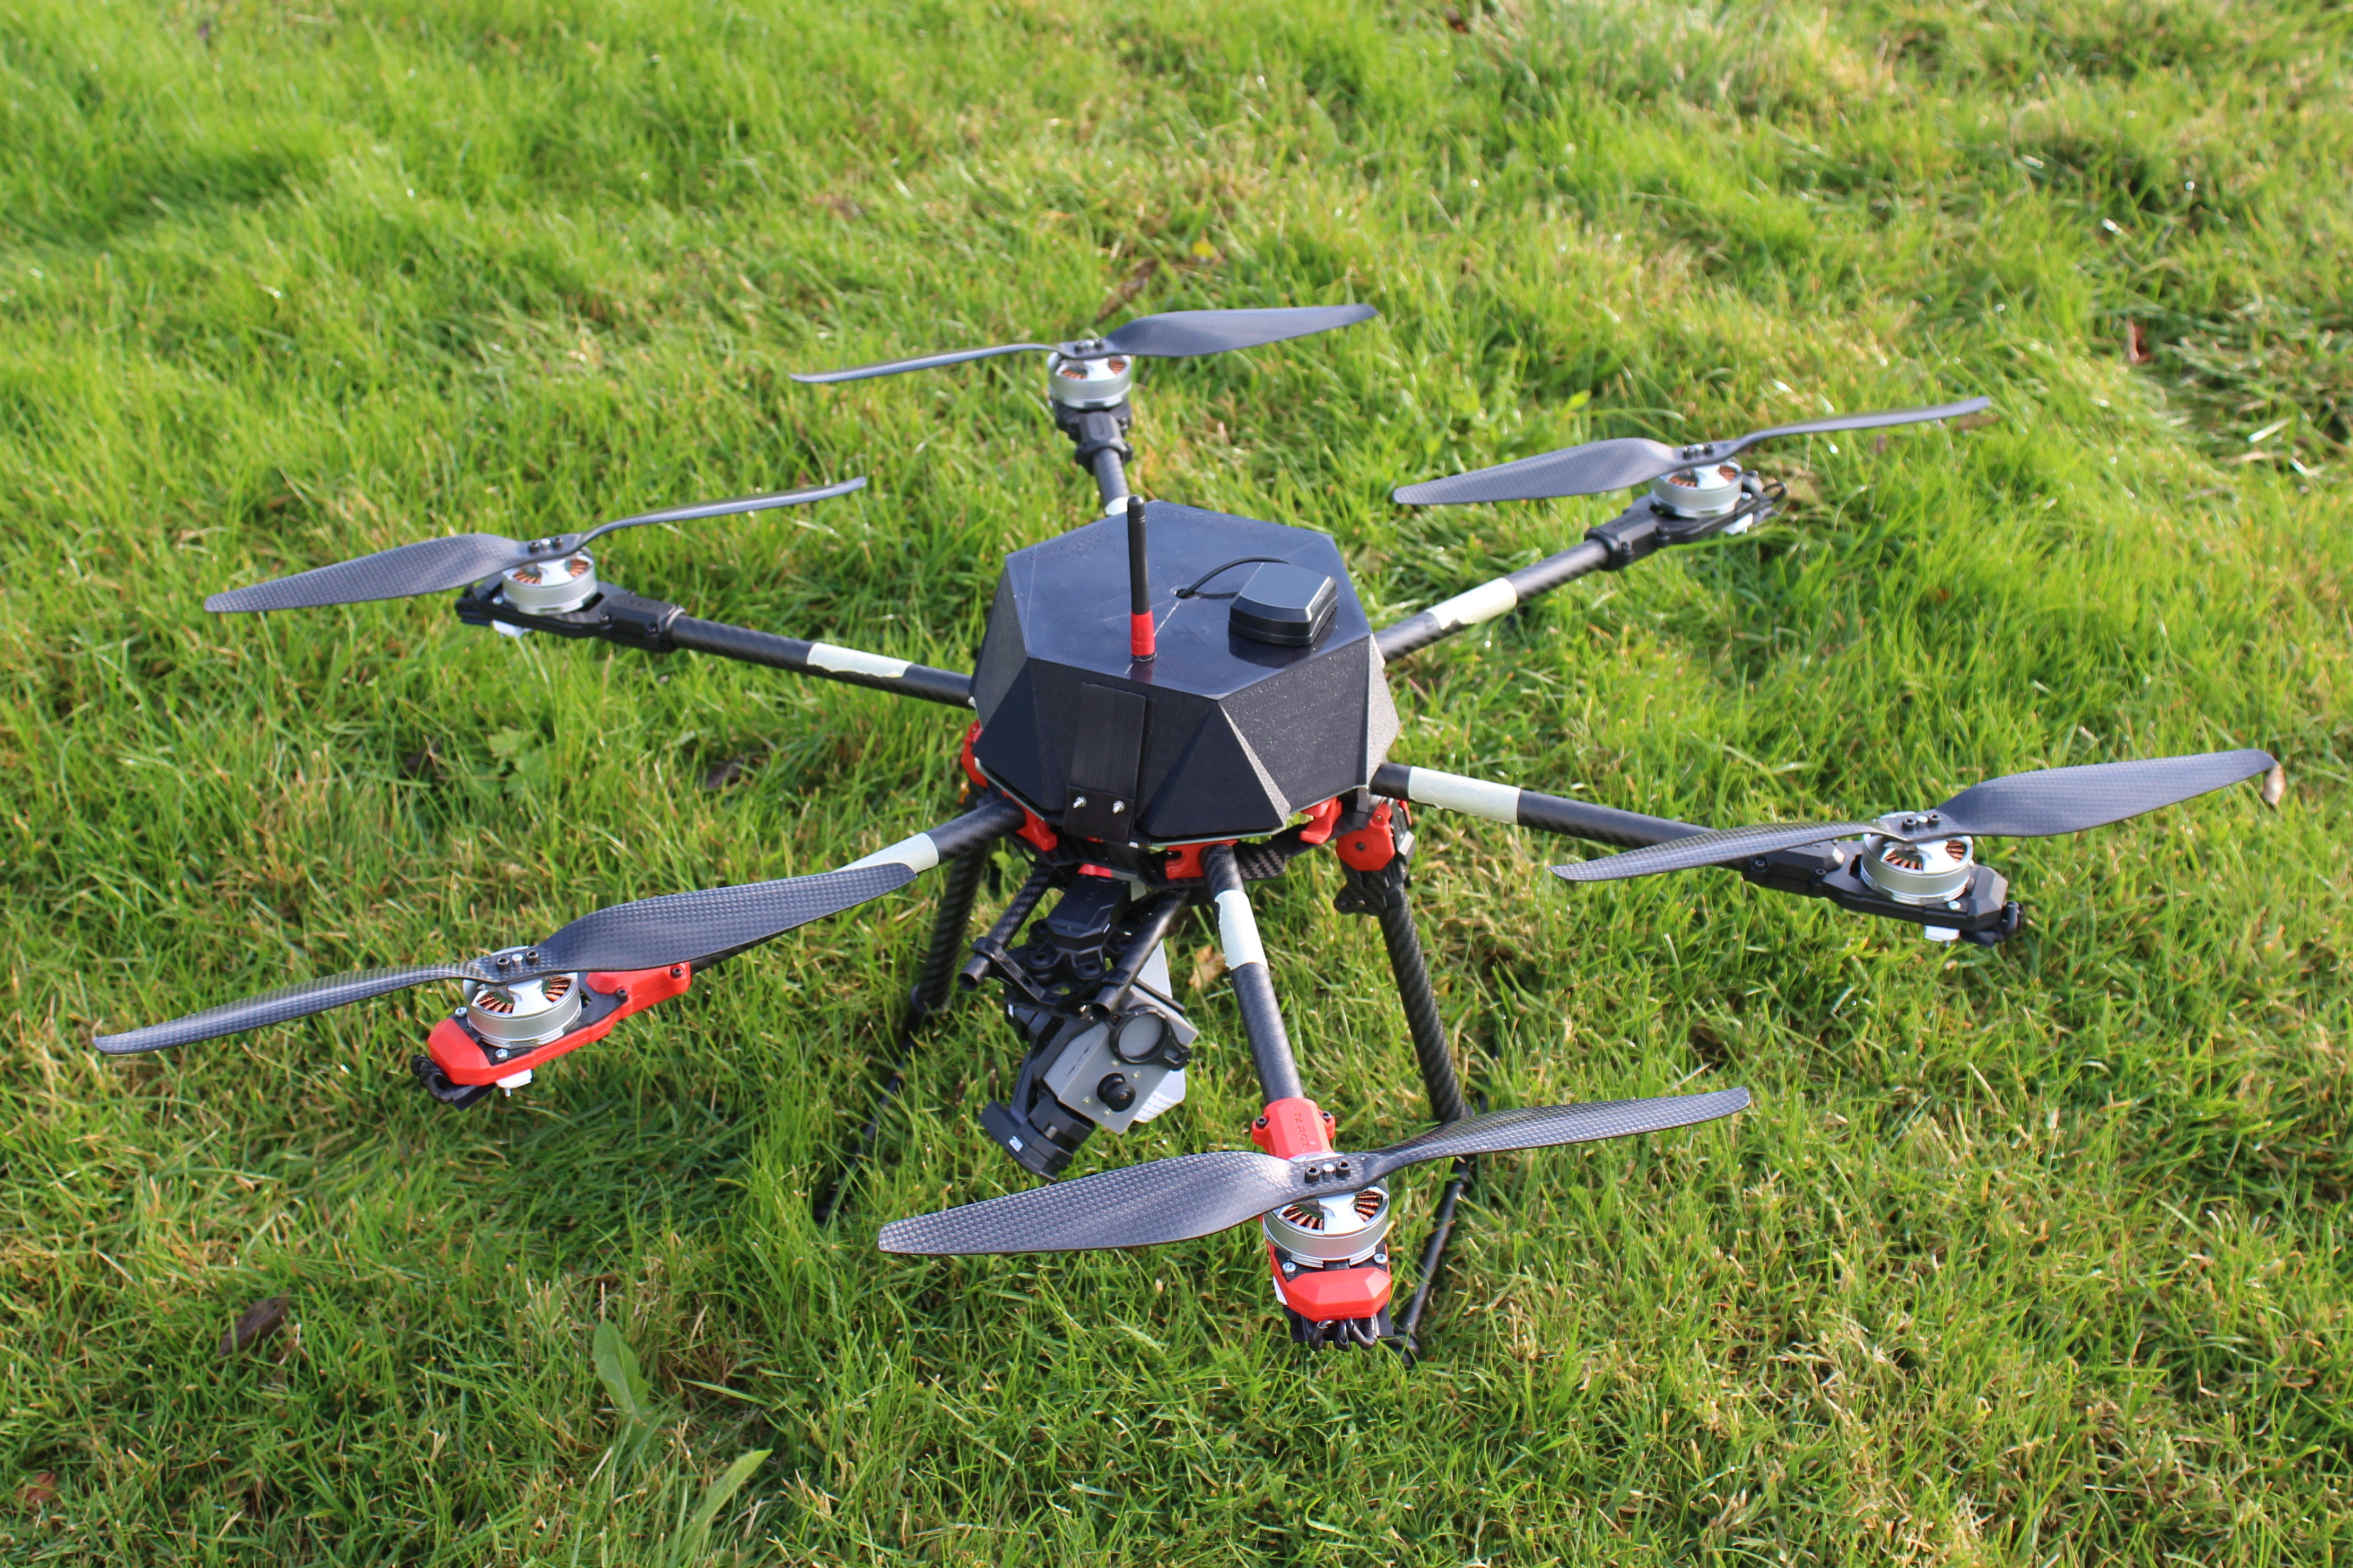
\includegraphics[width=\textwidth]{images/jetson_drone.JPG}
        \caption{The Jetson drone.}
        \label{fig:jetson_drone}
    \end{subfigure}
    \begin{subfigure}[b]{0.48\textwidth}
        \centering
        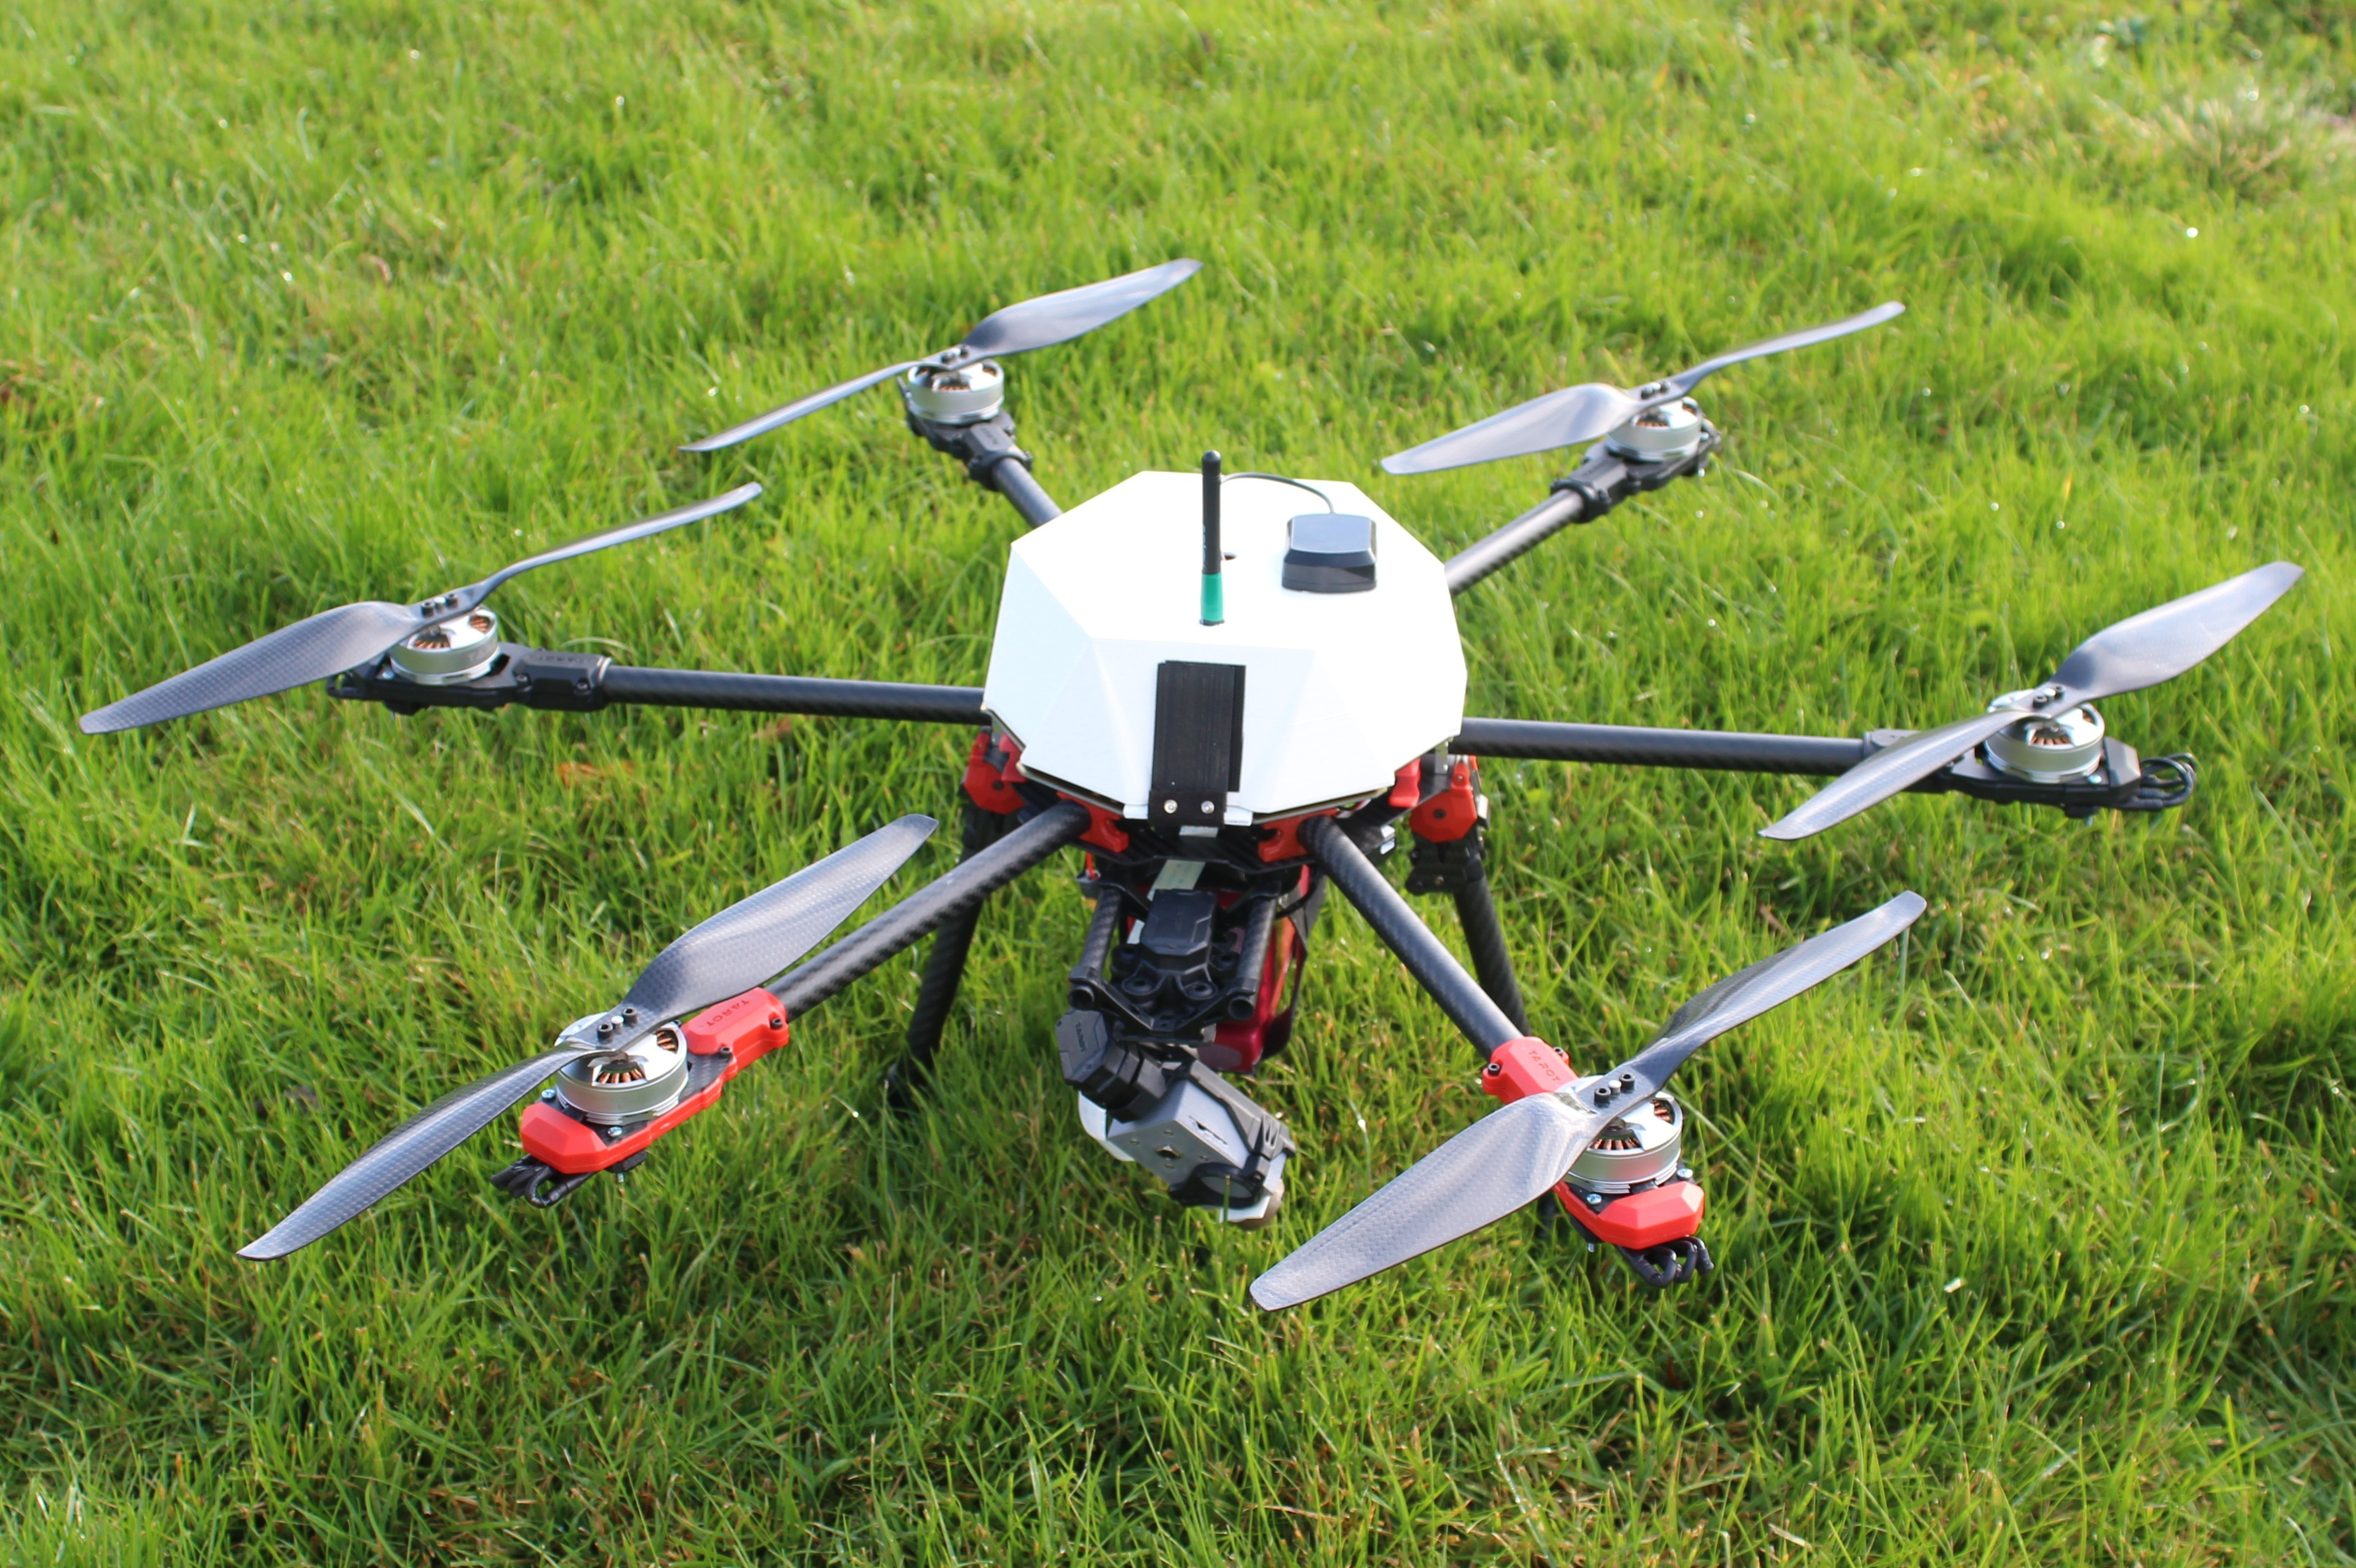
\includegraphics[width=\textwidth]{images/coral_drone.JPG}
        \caption{The Coral drone.}
        \label{fig:coral_drone}
    \end{subfigure}
    
    \begin{subfigure}[b]{0.48\textwidth}
        \centering
        \includegraphics[width=\textwidth]{images/jetson_electronics.JPG}
        \caption{The Jetson drone's electronics compartment.}
        \label{fig:jetson_electronics}
    \end{subfigure}
    \begin{subfigure}[b]{0.48\textwidth}
        \centering
        \includegraphics[width=\textwidth]{images/coral_electronics.JPG}
        \caption{The Coral drone's electronics compartment.}
        \label{fig:coral_electronics}
    \end{subfigure}
    
    \caption{The assembled drones and their electronics compartments.}
    \label{fig:drone_pictures}
\end{figure}

\subsection{Automatic Gimbal Aiming}

The performance of the gimbal controller to aim the camera at the marker was tested first in a lab environment. The drone was left still, and the marker was initially positioned from at various points in the camera's view. The camera's view of the marker was obscured so that the gimbal would aim at an idle point, directly in front of the drone. Then, while the marker was kept in a static location, the camera's view was unblocked and the position of the marker in the camera's frame was recorded for 10 seconds. The results for the Jetson drone are presented in Figures \ref{fig:jetson_gimbal_performance_x_axis} and \ref{fig:jetson_gimbal_performance_y_axis}, and the results for the Coral drone are presented in Figures \ref{fig:coral_gimbal_performance_x_axis} and \ref{fig:coral_gimbal_performance_y_axis}. In order to achieve reliable results, the maximum angular speed of the gimbal was reduced to 100 deg/s in all axes. This gives the PID controllers adequate time to adjust their control effort outputs, and decreases motion blur in the video stream, allowing easier recognition of the marker.

As shown in Figure \ref{fig:jetson_gimbal_performance_x_axis}, the gimbal is able to keep the marker in view from a range of starting points, and moves the camera towards the marker in the x axis. While many of the lines center the marker at a position of 320 (out of 640) pixels, some of the lines do not approach this value. This is because the angular range of the gimbal was limited to $\pm$30 degrees in the x axis, and the marker was more than 30 degrees offset from the center of the camera when it was at its extreme position. This is acceptable because of the 160\degree field of view of the Jetson's camera module. In Figure \ref{fig:jetson_gimbal_performance_y_axis}, the performance of the gimbal controller in the y axis is shown. The gimbal is limited to $[-90, 10]$ in the y axis, and it is able to center the marker in the camera frame for all starting points. Low PID coefficients were chosen, providing slow, smooth correction, which again is possible because of the camera module's wide field of view.

Since the Google Coral's camera module has a smaller field of view, the PID settings were configured to cause very quick adjustment of the camera's position upon finding the marker. Although this resulted in some oscillation which is visible in Figures \ref{fig:coral_gimbal_performance_x_axis} and \ref{fig:coral_gimbal_performance_y_axis}, the camera is still able to track the marker successfully. Smaller PID coefficients sometimes result in a loss of the marker if the marker moves too fast, while other configurations result in diverging oscillation. The integral gain is particularly useful for slow, smooth control, but does cause oscillation if set too high, so it was kept as high as possible while removing \textit{divergent} oscillation. However, since it was not sufficiently high, the camera does not fully center the marker for large negative angles which correspond to the lines that do not converge to near $v=240$. This is acceptable because the marker still stays in the frame of the camera.

Ultimately the method for aiming the gimbal is successful. Moreover, in-motion tracking of the marker gives consistent and smoother results, without oscillation. Still, more sophisticated controllers than PID controllers could improve performance.

\begin{figure}
    \centering
    \begin{subfigure}[b]{0.49\textwidth}
        \centering
        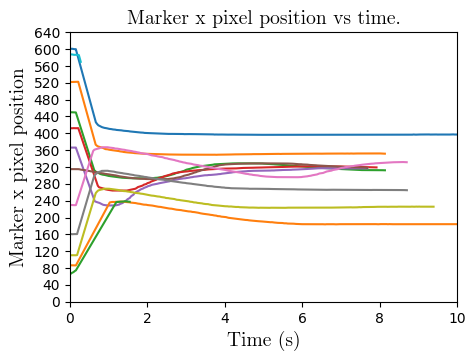
\includegraphics[width=\textwidth]{images/jetson_gimbal_performance_x_axis.png}
    \caption{Performance of the Jetson drone aiming the gimbal in the x axis.}
    \label{fig:jetson_gimbal_performance_x_axis}
    \end{subfigure}
    \begin{subfigure}[b]{0.49\textwidth}
        \centering
        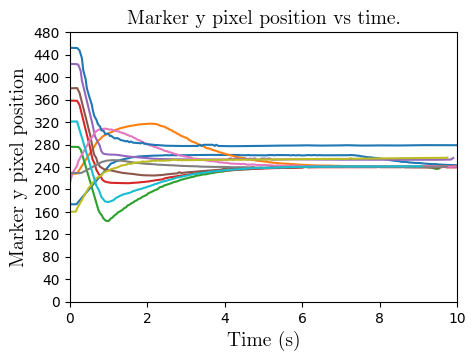
\includegraphics[width=\textwidth]{images/jetson_gimbal_performance_y_axis.png}
    \caption{Performance of the Jetson drone aiming the gimbal in the y axis.}
    \label{fig:jetson_gimbal_performance_y_axis}
    \end{subfigure}
        \begin{subfigure}[b]{0.49\textwidth}
        \centering
        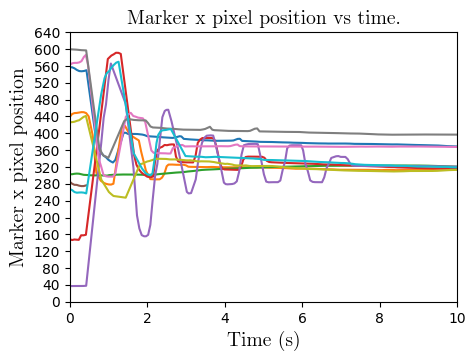
\includegraphics[width=\textwidth]{images/coral_gimbal_performance_x_axis.png}
    \caption{Performance of the Coral drone aiming the gimbal in the x axis.}
    \label{fig:coral_gimbal_performance_x_axis}
    \end{subfigure}
    \begin{subfigure}[b]{0.49\textwidth}
        \centering
        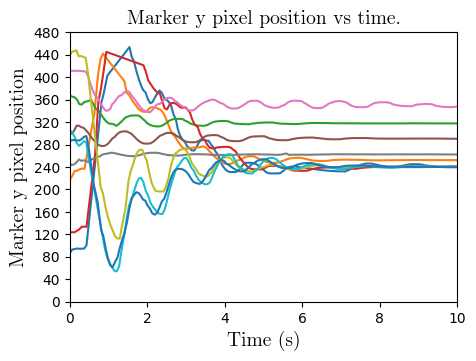
\includegraphics[width=\textwidth]{images/coral_gimbal_performance_y_axis.png}
    \caption{Performance of the Coral drone aiming the gimbal in the y axis.}
    \label{fig:coral_gimbal_performance_y_axis}
    \end{subfigure}
    \caption{Performance of aiming the gimbals.}
    \label{fig:gimbal_aim_performance}
\end{figure}

% \begin{figure}
%     \centering
%     \includegraphics[width=0.9\textwidth]{images/gimbal_performance_x_axis.png}
%     \caption{Performance of aiming the gimbal in the x axis.}
%     \label{fig:gimbal_performance_x_axis}
% \end{figure}

% \begin{figure}
%     \centering
%     \includegraphics[width=0.9\textwidth]{images/gimbal_performance_y_axis.png}
%     \caption{Performance of aiming the gimbal in the y axis.}
%     \label{fig:gimbal_performance_y_axis}
% \end{figure}

\subsection{Flight Performance}
\subsubsection{Maiden Flights}
% For our first flight, after finding a suitable location, we flew with manual control in order to test the PID controls on ArduCopter. We hovered the drone close to the ground and ran through all of the potential maneuvers it would need to complete. The stock PID configurations were very much adequate in all pitch, roll, yaw, and throttle inputs, responding quite well. After landing we went over the drone again to check the condition of everything, and confirmed that everything was still fine. After the test, which was conducted over two minutes, we found that it had used 700mah out of 10,000.

% The maiden flights of each drone were quite successful. The stock PID settings in the ArduPilot software were adequate for stable flight, even in winds of 5-10 m/s. The 
The first flights of each drone were conducted over about 2 minutes each. Both drones performed satisfactorily with basic hovering, horizontal and vertical movement, and yawing. The stock ArduPilot PID controller configurations on every axis provided reliable control with no oscillation. The drones were able to hold their positions in space even in the presence of wind. The frames were robust in both flight and landing. The energy used for each of the 2-minute flights was about 700 mAh from a total capacity of 10,000 mAh on the larger battery. This energy consumption rate was similar to all subsequent flights.

\subsubsection{Stability}
One of the main tasks of drone flight is simply to hover. Figure \ref{fig:hover_performance} illustrates the performance of the drone in hovering for 30 seconds. It is able to maintain its orientation in the pitch and roll axes quite well, even while changing altitude. The mean and standard deviation for the pitch and roll values during these 30 seconds are shown in Table \ref{tab:attitude}. The included video ``Initial Drone Flights'' provides a more intuitive way to view the stability of the drone's flight performance.\footnote{``Initial Drone Flights'' video: \url{https://vimeo.com/461576798}}

\begin{figure}
    \centering
    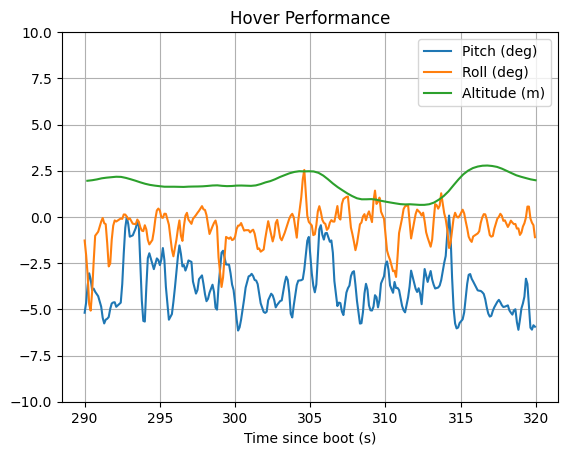
\includegraphics[width=0.7\textwidth]{images/stability.png}
    \caption{Attitude and altitude of the drone during 30 seconds of hovering.}
    \label{fig:hover_performance}
\end{figure}

\begin{table}
    \centering
    \begin{tabular}{|c|c|c|}
    \hline
        \textbf{Data} & \textbf{Mean} & \textbf{Standard Deviation} \\\hline
        Pitch & -3.79\degree & 1.37\degree \\\hline
        Roll & -0.53\degree & 0.98\degree \\\hline
    \end{tabular}
    \caption{Attitude while hovering.}
    \label{tab:attitude}
\end{table}

\subsubsection{Initial Landing Attempts}
The initial landing attempts were conducted as follows. A pilot manually hovered the drone over the landing pad in order to provide the drone with a view of the WhyCon marker. Visual acquisition of the marker was verified simply by ensuring that the gimbal was changing orientation to aim the camera at the landing pad. After visual acquisition was confirmed, the drone was placed from ``STABILIZE'' mode into ``GUIDED'' mode, enabling the landing controller to command the drone using positional targets.

The first attempts were made with the Jetson Nano drone (as shown in Figure \ref{fig:jetson_in_flight}), whose power issues prevented reliable visual acquisition of the landing pad. Although the drone was able to successfully hover and all components except for the Jetson Nano ran without problems, the landing attempts ultimately had to be delayed until these issues are fixed.

\begin{figure}
    \centering
    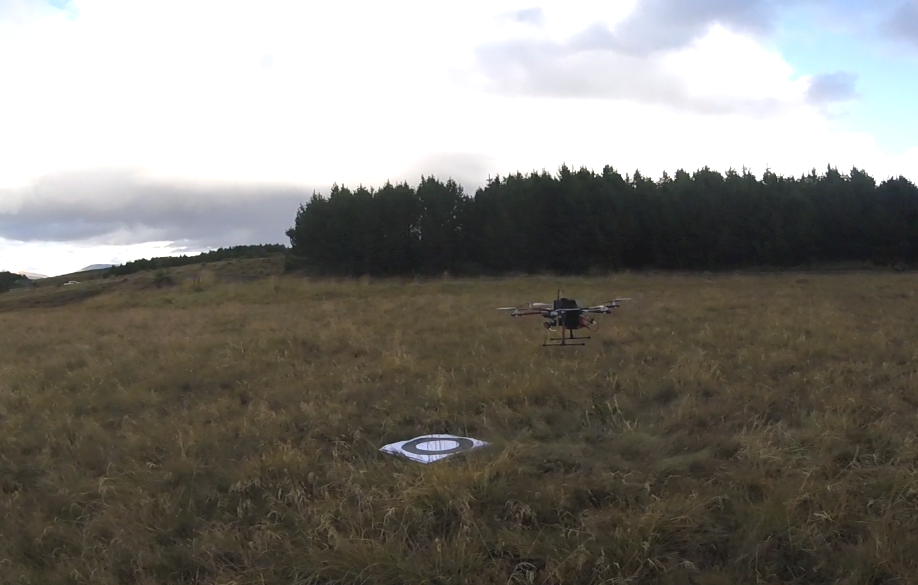
\includegraphics[width=0.75\textwidth]{images/drone_in_flight.png}
    \caption{The Jetson drone in flight.}
    \label{fig:jetson_in_flight}
\end{figure}

The next attempts were made with the Google Coral drone. This drone was able to successfully identify and track the landing pad in flight. Upon switching to ``GUIDED'' mode, the drone successfully approached the landing pad in the plane and decreased its height. However, because of a combination of factors, the final touchdown was not successful. First the region of allowable descent was too tight, meaning that the drone would have to land in an area defined by a 30cm radius. This by itself is not a problem, but becomes a problem because of the inaccuracies in pose estimation when the marker is viewed from extreme angles: the magnitude of the pose becomes smaller than in actuality, meaning that a small positional drift by the drone can be perceived as a prohibitively large positional drift. Essentially, the drone perceives itself as outside of the descent region and attempts to correct its horizontal position before descending. Moreover, there is another phenomenon at play called the ``ground effect.'' This occurs when the drone is close enough to the ground that the air pushed by the propellers bounces off the ground and produces a secondary thrust effect, changing the dynamics of the system \cite{ground_effect_article}. It is harder for the drone to maintain its position when it is close to the ground because of this extra turbulence. Therefore, although the drone successfully approached the landing pad, attained an acceptable horizontal position for landing, and descended to only about 5-10 centimeters from the ground, it never fully reached the ground autonomously.

All of these issues represent surmountable challenges only, and specifically \textit{not} prohibitive obstacles. They can be solved with iterative adjustment of the landing control policy and re-calibration of the WhyCon system, as well as possible filtering of the position of the landing pad. However, the limited time for a summer project means that this is not yet accomplished. It is part of our future work. So far, we have carried out 6 testing attempts, with multiple flights per attempt. These were conducted just east of Reykjavik.

\section{Discussion}


% \subsection{Practical Challenges}
\subsection{Supply Chain Issues}

The Tarot 680 kit uses 28mm M2.5 machine screws which are atypical for Iceland and could not be found. Moreover, half of such necessary screws were missing from the drone kits (4 missing for each drone). This meant that only one drone could initially be assembled until a colleague graciously retrieved some acceptable 30mm M2.5 machine screws from mainland Europe.

The Google Coral camera module uses a smaller ribbon cable than those compatible with the Raspberry Pi and similar boards. The short ribbon cable that comes with the camera module is unusable in this application because it does not allow the gimbal to move freely throughout its entire range of motion. To solve this, several terminals were delicately removed by hand from an existing, longer cable with the same terminal size. This cable was then successfully used both in the lab and the field to provide good connectivity between the Google Coral and its camera module.

In general, the main connector used between components is a USB cable. However, the small electronics compartment and the large number of components sitting therein meant that a lot of these cables had to be modified to fit with the canopy completely closed. The stiff, plastic ends of some of these cables were cut in order to make them take up less room, particularly in the case of the Jetson Nano whose micro USB port was quite close to the canopy walls. Additionally, many of these cables were shortened by cutting and re-soldering the wires to reduce space and weight.

\subsection{ROS Installation}

Installing the ROS software stack on the Jetson Nano and Google Coral can be a challenge because of the number of dependencies and the specific operating systems which do not have as much popularity as typical Linux distributions that ROS targets, such as basic Ubuntu. Significant time was spent creating reliable installation instructions for both boards. Such instructions were a necessary step, as a single working OS image is not adequate for the project since SD cards or installations may otherwise fail, and the system may need to be reinstalled. On-board compilation of ROS sources takes a long time but is ultimately not prohibitively time-consuming.

The Jetson Nano runs a modified version of Ubuntu 18.04 called Tegra, which comes with a lot of desktop applications and games that were removed prior to the installation of ROS. These take up a large portion of the system image that is provided by NVIDIA, and they are completely unnecessary. Many of the necessary ROS modules use OpenCV, but are incompatible with OpenCV 4 which is provided on this system image. Therefore, OpenCV was downgraded to version 3.2 for compatibility. Many of the ROS dependencies can be installed through the Aptitude package manager on this board, but the \texttt{whycon\_ros}, \texttt{jetson\_csi\_cam}, \texttt{gscam}, \texttt{gimbal\_controller}, and \texttt{landing\_controller} modules were necessarily installed from source. After many attempts at installation, with multiple ROS distributions, this method of combining binary and source installations worked on the board with the Melodic ROS distribution.

The Google Coral runs a modified version of Ubuntu 18.04 called Mendel Linux, which is much more lightweight than Tegra. The Coral's 8 GB of fast, onboard storage means that the Coral runs generally more smoothly and boots more quickly than the Jetson Nano, which boots from an SD card. However, an SD card was eventually needed for the ROS installation. This installation was done entirely from source, although some binaries are provided through Aptitude. A swap file is needed both for ROS installation and initialization.

The ROS Melodic distribution was successfully installed on both boards, using dependencies for Ubuntu 18.04 by setting the \texttt{ROS\_OS\_OVERRIDE} environment variable to \texttt{ubuntu:18.04:bionic}.

\subsection{Jetson Nano Power Consumption and Form Factor}
\label{section:jetson_nano_power_consumption_and_form_factor}

Although the Jetson Nano itself can run without a problem given the setup of the electronic system onboard its drone, the camera adds too much to the power requirements. The result is that the Jetson Nano is unable to sustain operation reliably. Although in lab scenarios it is generally able to successfully identify the landing pad, aim the gimbal, and generate a positional target based on the landing pad's pose, it tends to shut off when the computational load becomes high. Moreover, the shutoff is akin to a brown-out in that the system voltage gradually decreases until the board no longer functions. This led to the failure of multiple SD cards which the board uses as its main storage and boot disk. A lot of overhead hours were spent identifying this issue and determining eventually that the Jetson Nano is not suited for this application because of its power requirements.

The relatively large form factor of the Jetson Nano also means that it takes up a lot of valuable space in the electronics compartment - both horizontally on the mounting plate, and vertically towards the top of the canopy (as shown in Figure \ref{fig:jetson_electronics}). This is especially so when using the recommended fan which mounts on top of the heat sink, which already takes up significant space.

\subsection{Gimbal Quirks}

The Tarot T-3D gimbal, used on both drones, is made for a Go Pro and calibrated for its weight. The 3D-printed camera cases and their mounted modules ware significantly lighter than a GoPro, and therefore created a weight imbalance in the roll axis of the gimbal, resulting in a higher-than-normal idle load on the gimbal roll motor. Conceptually this is not a problem, as the gimbal is still able to hold the camera smooth when the gimbal's IMU senses vibration or other movement. However, in static testing, the gimbal detects this higher effort and temporarily shuts off in order to attempt to save the gimbal. Normally the higher effort would correspond to some physical block to the gimbal's motion, and there is a risk of burning out the motor if current is continuously applied. To work around this behavioral quirk, and the closed source, black box gimbal firmware, additional weight was added to the camera case for balance.

Although the gimbal does calculate its orientation and can provide it to its firmware GUI on a Windows machine, it does not provide its orientation as data through an interface that can be read by the flight controller. Although it is theoretically possible to reverse-engineer the communication between the gimbal firmware and its IMU, this task is beyond the scope of the project and has the potential to be extremely time-consuming. A first attempt to estimate the gimbal's pan and tilt angles was moderately successful, as explained in Section \ref{section:gimbal_controller_adapation}. However, this attempt was ultimately abandoned because, although a simple PWM signal does communicate a target angle to the gimbal, the gimbal only approaches this angle over a non-negligible amount of time using its own PID controllers. This means that, if the gimbal controller calculates an angle based on the PWM signal that is sending to the gimbal, that calculated angle will have some non-negligible, transient error if the drone or the gimbal is in motion. Since both the drone and the gimbal are constantly in motion in the flight scenarios of this project, determination of the gimbal's orientation is avoided, and all pose estimation is done strictly from the pose of the WhyCon marker on the landing pad. Additionally, since the marker has no reliable yaw orientation, the pan (yaw) axis of the gimbal is fixed straight ahead via a static PWM signal.

\subsection{Field Testing Restrictions and Environmental Limitations}

A conservative testing methodology addresses the high risk of drone flight generally, as well as material scarcity and restrictions on drone flight at the campus of Reykjavik University. Testing was conducted outside the city of Reykjavik, and away from the airport, meaning that all flights were extremely focused with a clear objective, in order to reduce the risk of expensive and time-consuming crashes, battery consumption and travel overheads. In-lab testing was maximized. The prevalence of high winds and rainy days significantly limited the available testing time. Even on calmer days, overcast skies significantly decreased GPS accuracy and therefore manual control was very important.

\section{Conclusion}
This project has demonstrated that fiducial markers can be used in combination with a gimbal-mounted camera to localize and approach a landing pad reliably, even without knowing the orientation of the gimbal. It is a proof of concept of many of the points addressed in simulation in the original thesis \cite{AL_thesis}. While more testing is needed to determine a better landing policy, and more development is needed for the WhyCode marker, nonetheless we have succeeded in building a drone that is capable of both manual and autonomous flight, real-time video analysis, and fiducial marker identification and tracking.

We have started communication with the maintainers of WhyCode in the Czech Republic and will continue to integrate WhyCode markers into our system. We will also adjust the landing control policy to reflect new knowledge of the performance of the drones during landing, and this will allow us to carry out successful landings in the near future. We will also focus on solving the power issues experienced with the Jetson Nano. Eventually we will test new methods of pose estimation and control, with a focus on artificial intelligence and machine learning.

\bibliographystyle{IEEEtran}
\bibliography{sections/references}

\end{document}